\documentclass[aspectratio=169, 12pt]{beamer}
\usepackage[UTF8]{ctex}
\usepackage{graphicx}
\usepackage{booktabs}
\usepackage{listings}
\usepackage{xcolor}
\usepackage{tikz}
\usetikzlibrary{shapes.geometric, arrows, positioning, calc}
\usepackage{amsmath}
\usepackage{hyperref}

% 修复 beamer verbatim 问题
\makeatletter
\def\verbatim@font{\normalfont\ttfamily}
\makeatother

% --- 主题风格 ---
\usetheme{Madrid}
\usecolortheme{whale}
\usefonttheme{professionalfonts}

% --- 代码高亮设置 ---
\lstset{
    language=Python,
    basicstyle=\ttfamily\small,
    keywordstyle=\color{blue},
    commentstyle=\color{green!60!black},
    stringstyle=\color{orange},
    breaklines=true,
    frame=single,
    showstringspaces=false,
    backgroundcolor=\color{gray!5}
}

% --- 自定义命令 ---
\newcommand{\highlight}[1]{\textcolor{red}{\textbf{#1}}}

\title[CV导论与图像基础]{第1周:计算机视觉导论与图像基础}
\subtitle{让机器“看懂”试卷的第一步}
\author{计算机视觉课程组}
\date{2024-2025 学年}

\begin{document}

% -----------------------------------------------------------------------------
% 标题页
% -----------------------------------------------------------------------------
\begin{frame}[fragile]{课程标题}
    \titlepage
\end{frame}

% -----------------------------------------------------------------------------
% 环节一:课程导论 (40分钟)
% -----------------------------------------------------------------------------
\section{计算机视觉导论}

\begin{frame}[fragile]{视觉:人类获取信息的最主要渠道}
    \begin{columns}
        \column{0.5\textwidth}
        \textbf{人类视觉:}
        \begin{itemize}
            \item 人脑约 50\% 的神经元参与视觉处理。
            \item \highlight{语义理解}:我们看到的不是像素,是“人”、“车”、“试卷”。
        \end{itemize}
        \vspace{0.5cm}
        \textbf{计算机视觉 (CV):}
        \begin{itemize}
            \item 目标:给机器安装“眼睛”和“大脑”。
            \item 挑战:图像在计算机眼中只是一组 \highlight{数字}。
        \end{itemize}

        \column{0.5\textwidth}
        \begin{figure}
            \centering
            \includegraphics[width=0.8\textwidth]{example-image}
            \caption{语义 vs 矩阵}
        \end{figure}
    \end{columns}
\end{frame}

\begin{frame}[fragile]{CV 的历史与现状}
    \begin{itemize}
        \item \textbf{1960s}:Larry Roberts (CV之父) 尝试让机器识别积木世界。
        \item \textbf{1970s-1980s}:提出边缘检测、Marr 视觉计算理论。
        \item \textbf{2012-至今}:\highlight{深度学习爆发},AlexNet 在 ImageNet 竞赛中夺冠。
    \end{itemize}
    \begin{block}{核心任务演变}
        分类 (是什么?) $\to$ 检测 (在哪儿?) $\to$ 分割 (形状如何?) $\to$ 生成 (画一个出来)
    \end{block}
\end{frame}

\begin{frame}[fragile]{贯穿本学期的项目:AI 阅卷助手}
    \begin{columns}
        \column{0.4\textwidth}
        \textbf{任务分解:}
        \begin{enumerate}
            \item \textbf{图像采集}:拍照、扫描。
            \item \textbf{预处理}:纠偏、增强(本周内容)。
            \item \textbf{定位}:找到答题卡、填空区。
            \item \textbf{识别}:OCR (光学字符识别)。
            \item \textbf{评分}:逻辑比对。
        \end{enumerate}
        \column{0.6\textwidth}
        \begin{center}
            \begin{tikzpicture}[scale=0.8]
                \draw[thick] (0,0) rectangle (4,5);
                \node at (2,4.5) {试卷图像};
                \draw[fill=blue!20] (0.5,3) rectangle (3.5,3.8); \node at (2,3.4) {学号区};
                \draw[fill=red!20] (0.5,1) rectangle (3.5,2.5); \node at (2,1.75) {答题区};
                \draw[->, ultra thick, red] (4.5, 2.5) -- (6, 2.5) node[right] {AI 识别};
            \end{tikzpicture}
        \end{center}
    \end{columns}
\end{frame}

% -----------------------------------------------------------------------------
% 新增:答题卡定位锚点(Timing Marks)
% -----------------------------------------------------------------------------

\begin{frame}[fragile]{项目深度:答题卡的"定位锚点" (Timing Marks)}
    \textbf{问题:}如果试卷皱了或者拍摄角度极度倾斜,如何准确定位答题卡?

    \begin{columns}
        \column{0.5\textwidth}
        \textbf{Timing Marks 的作用:}
        \begin{itemize}
            \item 答题卡边缘的黑色小方块
            \item 用于精确定位答题卡区域
            \item 类似二维码的定位图案
        \end{itemize}

        \vspace{0.3cm}
        \textbf{设计规范:}
        \begin{itemize}
            \item 位置:四个角或边缘
            \item 大小:固定的几何尺寸
            \item 对比度:黑色 vs 白纸
            \item 排列:特定模式(如L形)
        \end{itemize}

        \column{0.5\textwidth}
        \begin{center}
            \begin{tikzpicture}[scale=0.6]
                % 试卷边框
                \draw[thick] (0,0) rectangle (6,8);

                % 定位块(Timing Marks)
                \draw[fill=black] (0.2,0.2) rectangle (0.8,0.8);
                \draw[fill=black] (5.2,0.2) rectangle (5.8,0.8);
                \draw[fill=black] (0.2,7.2) rectangle (0.8,7.8);
                \draw[fill=black] (5.2,7.2) rectangle (5.8,7.8);

                % 标注
                \node[below] at (0.5,0.2) {\tiny 定位块};
                \node[above] at (5.5,7.8) {\tiny 定位块};

                % 答题区
                \draw[fill=blue!10] (1,2) rectangle (5,6);
                \node at (3,4) {答题区};

                % 箭头说明
                \draw[->, red, thick] (0.8,0.5) -- (2,0.5) node[right] {\tiny 检测黑块定位};
            \end{tikzpicture}
        \end{center}
    \end{columns}

    \vspace{0.3cm}
    \begin{block}{工程价值}
        Timing Marks 是阅卷系统的"眼睛",有了它们,即使试卷皱了也能准确定位
    \end{block}
\end{frame}

\begin{frame}[fragile]{定位锚点检测:从轮廓到坐标}
    \textbf{核心思路:}检测黑色方块 $\to$ 计算中心 $\to$ 透视变换

    \begin{columns}
        \column{0.5\textwidth}
        \begin{lstlisting}[language=Python, basicstyle=\ttfamily\tiny]
import cv2
import numpy as np

# 1. 读取答题卡
img = cv2.imread('answer_sheet.jpg')
gray = cv2.cvtColor(img, cv2.COLOR_BGR2GRAY)

# 2. 二值化
_, binary = cv2.threshold(gray, 127, 255,
                          cv2.THRESH_BINARY)

# 3. 查找黑色方块轮廓
contours, _ = cv2.findContours(
    binary, cv2.RETR_EXTERNAL,
    cv2.CHAIN_APPROX_SIMPLE
)

# 4. 筛选定位块(小方块)
marks = []
for cnt in contours:
    area = cv2.contourArea(cnt)
    # 定位块面积通常在特定范围
    if 100 < area < 1000:
        # 计算中心点
        M = cv2.moments(cnt)
        if M['m00'] != 0:
            cx = int(M['m10'] / M['m00'])
            cy = int(M['m01'] / M['m00'])
            marks.append((cx, cy))

print(f"检测到 {len(marks)} 个定位点")
        \end{lstlisting}

        \column{0.5\textwidth}
        \textbf{检测流程:}
        \begin{enumerate}
            \item \textbf{二值化}:
            \begin{itemize}
                \item 分离黑色定位块和白色背景
            \end{itemize}
            \item \textbf{轮廓查找}:
            \begin{itemize}
                \item 找到所有黑色区域
            \end{itemize}
            \item \textbf{面积筛选}:
            \begin{itemize}
                \item 定位块面积固定
                \item 排除过大或过小的轮廓
            \end{itemize}
            \item \textbf{中心计算}:
            \begin{itemize}
                \item 使用质心矩计算中心点
                \item 得到精确定位坐标
            \end{itemize}
        \end{enumerate}

        \vspace{0.2cm}
        \textbf{下一步(下周预告):}
        \begin{itemize}
            \item 透视变换:矫正倾斜
            \item 特征匹配:自动定位
        \end{itemize}
    \end{columns}
\end{frame}

\begin{frame}[fragile]{引出下周:透视变换的力量}
    \textbf{场景:}检测到定位点后,如何矫正倾斜的试卷?

    \begin{columns}
        \column{0.5\textwidth}
        \textbf{当前问题:}
        \begin{itemize}
            \item 手机拍照难免倾斜
            \item 试卷可能有透视变形
            \item 直接处理会降低识别率
        \end{itemize}

        \vspace{0.3cm}
        \textbf{下周解决方案:}
        \begin{enumerate}
            \item \textbf{透视变换}:
            \begin{itemize}
                \item 将任意四边形矫正为矩形
                \item 需要4个角点坐标
            \end{itemize}
            \item \textbf{特征匹配}:
            \begin{itemize}
                \item 自动找到定位点
                \item 无需人工标注
            \end{itemize}
        \end{enumerate}

        \vspace{0.3cm}
        \textbf{真实效果:}
        \begin{itemize}
            \item 任意角度拍摄 $\to$ 完美正面视图
            \item 像用扫描仪扫描一样
        \end{itemize}

        \column{0.5\textwidth}
        \begin{center}
            \begin{tikzpicture}[scale=0.5]
                % 原始倾斜图像
                \begin{scope}[shift={(0,0)}]
                    \draw[thick, fill=gray!20] (0,0) -- (3,1) -- (4,5) -- (1,4) -- cycle;
                    \node at (2,2.5) {\tiny 倾斜试卷};
                    % 定位点
                    \fill[black] (0.2,0.3) circle (0.1);
                    \fill[black] (2.8,1.2) circle (0.1);
                    \fill[black] (3.8,4.7) circle (0.1);
                    \fill[black] (1.2,3.8) circle (0.1);
                \end{scope}

                % 箭头
                \draw[->, ultra thick, blue] (4.5,2.5) -- (6.5,2.5) node[midway,above] {\tiny 透视变换};

                % 矫正后图像
                \begin{scope}[shift={(7,0)}]
                    \draw[thick, fill=white] (0,0) rectangle (4,5);
                    \node at (2,2.5) {\tiny 矫正面};
                    % 定位点
                    \fill[black] (0.2,0.2) rectangle (0.5,0.5);
                    \fill[black] (3.5,0.2) rectangle (3.8,0.5);
                    \fill[black] (0.2,4.5) rectangle (0.5,4.8);
                    \fill[black] (3.5,4.5) rectangle (3.8,4.8);
                \end{scope}
            \end{tikzpicture}
        \end{center}

        \vspace{0.5cm}
        \begin{block}{关键技术}
        \texttt{cv2.getPerspectiveTransform()} + \texttt{cv2.warpPerspective()}\\
        这两个函数是阅卷系统定位的核心!
        \end{block}
    \end{columns}
\end{frame}

% -----------------------------------------------------------------------------
% 环节二:图像的数字表示 (50分钟)
% -----------------------------------------------------------------------------
\section{图像的数字表示}

\begin{frame}[fragile]{图像的底层本质:矩阵 (Matrix)}
    \begin{columns}
        \column{0.5\textwidth}
        \begin{itemize}
            \item 一张灰度图 = 一个 \textbf{二维矩阵}。
            \item 矩阵中的每个元素称为 \highlight{像素 (Pixel)}。
            \item 常用数据类型:\texttt{uint8} (0-255)。
        \end{itemize}
        \column{0.5\textwidth}
        \begin{center}
            \small
            $\begin{bmatrix}
            255 & 255 & 254 \\
            120 & 0 & 118 \\
            255 & 253 & 255
            \end{bmatrix}$
            \vspace{0.2cm}
            \\ (矩阵数值 $\to$ 图像亮度)
        \end{center}
    \end{columns}
    \begin{alertblock}{注意坐标系!}
        计算机图像坐标系:\textbf{左上角为原点 (0,0)},X轴向右,Y轴向 \highlight{下}。
    \end{alertblock}
\end{frame}

\begin{frame}[fragile]{彩色图像:RGB 三通道}
    \begin{itemize}
        \item 彩色图像 = 三个二维矩阵堆叠 (\textbf{三维张量})。
        \item 每个通道代表一种颜色光的强度。
    \end{itemize}
    \begin{center}
        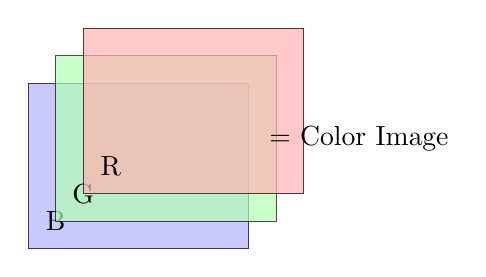
\begin{tikzpicture}[scale=0.7]
            \draw[fill=blue!30, opacity=0.7] (0,0) rectangle (4,3); \node at (0.5, 0.5) {B};
            \draw[fill=green!30, opacity=0.7] (0.5,0.5) rectangle (4.5,3.5); \node at (1, 1) {G};
            \draw[fill=red!30, opacity=0.7] (1,1) rectangle (5,4); \node at (1.5, 1.5) {R};
            \node at (6, 2) {= Color Image};
        \end{tikzpicture}
    \end{center}
    \textbf{OpenCV 的特殊性:} 默认读取顺序是 \highlight{BGR},而非 RGB。
\end{frame}

\begin{frame}[fragile]{互动练习:调色盘}
    如果一个像素的 RGB 值为以下数值,它是什么颜色?
    \begin{table}
        \centering
        \begin{tabular}{cccc}
            \toprule
            R & G & B & 预测颜色 \\
            \midrule
            255 & 255 & 0 & \uncover<2->{\textcolor{yellow}{黄色}} \\
            0 & 255 & 255 & \uncover<3->{\textcolor{cyan}{青色/浅蓝}} \\
            128 & 128 & 128 & \uncover<4->{\textcolor{gray}{灰色}} \\
            0 & 0 & 0 & \uncover<5->{\textbf{黑色}} \\
            \bottomrule
        \end{tabular}
    \end{table}
\end{frame}

% -----------------------------------------------------------------------------
% 新增:图像直方图理论
% -----------------------------------------------------------------------------

\begin{frame}[fragile]{图像的统计特性:直方图 (Histogram)}
    \begin{columns}
        \column{0.5\textwidth}
        \textbf{什么是直方图?}
        \begin{itemize}
            \item 横坐标:亮度级别 (0-255)
            \item 纵坐标:该亮度像素出现的频次
        \end{itemize}

        \vspace{0.3cm}
        \textbf{在阅卷中的意义:}
        \begin{itemize}
            \item \highlight{曝光检查}:判断照片是否太暗或过曝
            \item \highlight{二值化参考}:寻找波谷作为分割阈值
        \end{itemize}

        \column{0.5\textwidth}
        \begin{lstlisting}[language=Python, basicstyle=\ttfamily\tiny]
import cv2
import matplotlib.pyplot as plt

# 计算直方图
img = cv2.imread('exam.jpg',
                 cv2.IMREAD_GRAYSCALE)
hist = cv2.calcHist([img], [0], None,
                    [256], [0, 256])

plt.plot(hist)
plt.title('Pixel Intensity Distribution')
plt.show()
        \end{lstlisting}
        \begin{center}
            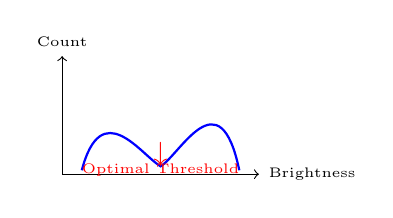
\begin{tikzpicture}[scale=0.5]
                \draw[->] (0,0) -- (5,0) node[right] {\tiny Brightness};
                \draw[->] (0,0) -- (0,3) node[above] {\tiny Count};
                \draw[thick, blue] (0.5,0.1) .. controls (1,2) and (2,0.5) .. (2.5,0.2) .. controls (3,0.5) and (4,2.5) .. (4.5,0.1);
                \node[red] at (2.5, 0.5) {$\downarrow$};
                \node[red, below] at (2.5, 0.5) {\tiny Optimal Threshold};
            \end{tikzpicture}
        \end{center}
    \end{columns}
\end{frame}

\begin{frame}[fragile]{直方图形态分析:试卷照片的曝光诊断}
    \textbf{场景:}自动判断试卷照片的质量

    \begin{columns}
        \column{0.5\textwidth}
        \textbf{1. 正常曝光(双峰分布)}
        \begin{itemize}
            \item 白纸(高亮度)+ 黑字(低亮度)
            \item 波谷在中间,适合二值化
            \item \textcolor{green!60!black}{\textbf{阅卷理想状态}}
        \end{itemize}

        \vspace{0.2cm}
        \textbf{2. 欠曝(左偏分布)}
        \begin{itemize}
            \item 大部分像素集中在暗部
            \item 可能是光照不足
            \item 需要亮度增强
        \end{itemize}

        \vspace{0.2cm}
        \textbf{3. 过曝(右偏分布)}
        \begin{itemize}
            \item 大部分像素集中在亮部
            \item 可能是闪光灯太强
            \item 需要降低亮度
        \end{itemize}

        \column{0.5\textwidth}
        \begin{lstlisting}[language=Python, basicstyle=\ttfamily\tiny]
def check_exposure(img):
    """检查图像曝光情况"""
    gray = cv2.cvtColor(img,
                       cv2.COLOR_BGR2GRAY)

    # 计算平均亮度
    mean_brightness = np.mean(gray)

    # 判断曝光状态
    if mean_brightness < 80:
        return "欠曝,建议增强"
    elif mean_brightness > 200:
        return "过曝,建议降低"
    else:
        return "曝光正常"

# 使用
status = check_exposure(img)
print(f"曝光状态: {status}")
        \end{lstlisting}
    \end{columns}
\end{frame}

\begin{frame}[fragile]{图像缩放:插值算法对比}
    \textbf{问题:}cv2.resize 时,像素是如何"凭空产生"或"消失"的?

    \begin{columns}
        \column{0.5\textwidth}
        \begin{lstlisting}[language=Python, basicstyle=\ttfamily\tiny]
import cv2
import numpy as np

img = cv2.imread('exam.jpg')
h, w = img.shape[:2]

# 1. 最近邻插值(最快)
# 取最近的像素值,会有马赛克
near = cv2.resize(img, (w*2, h*2),
                  interpolation=cv2.INTER_NEAREST)

# 2. 双线性插值(默认)
# 周围4个像素加权平均,较平滑
linear = cv2.resize(img, (w*2, h*2),
                   interpolation=cv2.INTER_LINEAR)

# 3. 双三次插值(最慢但最好)
# 周围16个像素加权平均
cubic = cv2.resize(img, (w*2, h*2),
                  interpolation=cv2.INTER_CUBIC)
        \end{lstlisting}

        \column{0.5\textwidth}
        \textbf{插值效果对比:}
        \begin{itemize}
            \item \textbf{最近邻}:
            \begin{itemize}
                \item 速度:最快
                \item 质量:有锯齿
                \item 应用:像素风游戏
            \end{itemize}
            \item \textbf{双线性}:
            \begin{itemize}
                \item 速度:中等
                \item 质量:较平滑
                \item 应用:日常缩放
            \end{itemize}
            \item \textbf{双三次}:
            \begin{itemize}
                \item 速度:最慢
                \item 质量:最平滑
                \item 应用:高质量缩放
            \end{itemize}
        \end{itemize}

        \vspace{0.2cm}
        \textbf{阅卷建议:}
        \begin{itemize}
            \item 缩小用 \texttt{INTER\_AREA}(抗锯齿)
            \item 放大用 \texttt{INTER\_CUBIC}(高质量)
        \end{itemize}
    \end{columns}
\end{frame}

% -----------------------------------------------------------------------------
% 环节三:OpenCV 入门 (40分钟)
% -----------------------------------------------------------------------------
\section{OpenCV 基础}

\begin{frame}[fragile]{OpenCV 核心函数详解}
    \begin{lstlisting}[title={图像读取的隐患}]
import cv2

# 路径千万不能有中文(新手常见错误)
img = cv2.imread('paper.jpg')

# 检查是否读取成功
if img is None:
    print("错误:文件不存在或路径含有中文!")

# 打印维度 (H, W, C)
print(img.shape)
    \end{lstlisting}
    \begin{block}{常用 Flag}
        \begin{itemize}
            \item \texttt{cv2.IMREAD\_COLOR}:加载彩色图(默认)。
            \item \texttt{cv2.IMREAD\_GRAYSCALE}:直接以灰度模式加载(节省内存)。
        \end{itemize}
    \end{block}
\end{frame}

% -----------------------------------------------------------------------------
% 新增:Unicode路径处理(避坑指南)
% -----------------------------------------------------------------------------

\begin{frame}[fragile]{工程实战:处理中文路径的"终极方案"}
    \begin{alertblock}{真实场景}
        阅卷系统中,学生姓名经常是中文,文件名如:\texttt{张三\_试卷.jpg}\\
        \texttt{cv2.imread()} 直接读取会失败(返回 None)
    \end{alertblock}

    \begin{columns}
        \column{0.5\textwidth}
        \textbf{问题原因:}
        \begin{itemize}
            \item OpenCV 的 C++ 库不支持 Unicode 路径
            \item 中文路径会乱码
            \item 这不是 Python 的问题,是 OpenCV 的限制
        \end{itemize}

        \vspace{0.3cm}
        \textbf{错误做法:}
        \begin{lstlisting}[language=Python, basicstyle=\ttfamily\tiny]
# 直接读取,返回 None
img = cv2.imread('张三_试卷.jpg')
if img is None:
    print("读取失败!")
        \end{lstlisting}

        \column{0.5\textwidth}
        \textbf{正确做法:}
        \begin{lstlisting}[language=Python, basicstyle=\ttfamily\tiny]
import cv2
import numpy as np

# 使用 np.fromfile + cv2.imdecode
def imread_chinese(path):
    """读取中文路径的图片"""
    # 从文件读取字节数据
    img_array = np.fromfile(path, dtype=np.uint8)

    # 解码为图像
    img = cv2.imdecode(img_array, -1)

    return img

# 使用
img = imread_chinese('张三_试卷.jpg')
cv2.imshow('成功!', img)
        \end{lstlisting}
    \end{columns}
\end{frame}

\begin{frame}[fragile]{工程实战:保存中文路径图片}
    \textbf{配套技巧:}保存时也支持中文路径

    \begin{columns}
        \column{0.5\textwidth}
        \begin{lstlisting}[language=Python, basicstyle=\ttfamily\tiny]
import cv2
import numpy as np

def imwrite_chinese(path, img):
    """保存中文路径的图片"""
    # 编码为字节数据
    is_success, img_buf = cv2.imencode(
        ".jpg", img
    )

    if is_success:
        # 保存到文件
        img_buf.tofile(path)
        return True
    return False

# 使用
img = cv2.imread('exam.jpg')
imwrite_chinese('处理结果_张三.jpg', img)
print("保存成功!")
        \end{lstlisting}

        \column{0.5\textwidth}
        \textbf{原理说明:}
        \begin{enumerate}
            \item \textbf{imdecode}:
            \begin{itemize}
                \item 从内存中的字节数组解码
                \item 绕过了文件系统的 Unicode 问题
            \end{itemize}
            \item \textbf{imencode + tofile}:
            \begin{itemize}
                \item 编码为字节数组
                \item 用 NumPy 的 tofile 写入
                \item 同样绕过了 Unicode 问题
            \end{itemize}
        \end{enumerate}

        \vspace{0.3cm}
        \textbf{阅卷系统应用:}
        \begin{itemize}
            \item 批量处理学生试卷
            \item 生成带学生姓名的结果文件
            \item 完全支持中文路径
        \end{itemize}
    \end{columns}
\end{frame}

\begin{frame}[fragile]{Matplotlib 显示与 BGR 转换}
    为什么用 \texttt{plt.imshow} 显示出来的人脸是青蓝色的?
    \begin{lstlisting}
import matplotlib.pyplot as plt

# OpenCV 是 BGR,Matplotlib 是 RGB
img_rgb = cv2.cvtColor(img, cv2.COLOR_BGR2RGB)

plt.imshow(img_rgb)
plt.show()
    \end{lstlisting}
    \textbf{思考:} 灰度图显示时需要设置 \texttt{cmap='gray'},否则会变成“原油色”。
\end{frame}

% -----------------------------------------------------------------------------
% 环节四:图像算术运算 (30分钟)
% -----------------------------------------------------------------------------
\section{图像滤镜原理}

\begin{frame}[fragile]{滤镜 1:灰度化 (Grayscale)}
    \textbf{为什么要灰度化?}
    \begin{itemize}
        \item 减少计算量(数据量降至 1/3)。
        \item 识别试卷上的文字,颜色信息通常是不必要的。
    \end{itemize}
    \textbf{原理:} $Gray = R \times 0.299 + G \times 0.587 + B \times 0.114$
    \\ (为什么绿色权重最高?因为人眼对绿色最敏感。)
\end{frame}

\begin{frame}[fragile]{滤镜 2:反色 (Inversion)}
    \textbf{原理:} $NewValue = 255 - OldValue$
    \begin{itemize}
        \item 黑色 (0) $\to$ 白色 (255)
        \item 白色 (255) $\to$ 黑色 (0)
    \end{itemize}
    \textbf{应用:} 增强暗背景下的试卷特征,或者扫描负片。
\end{frame}

\begin{frame}[fragile]{滤镜 3:亮度调整与“溢出”陷阱}
    \textbf{错误做法:} \texttt{img + 50}
    \\ 如果像素值是 220,加 50 变成 270。而在 \texttt{uint8} 类型下,270 会变成 \highlight{14} (截断/绕回),导致图像出现难看的噪点。

    \begin{lstlisting}[title={安全写法}]
# 使用 numpy 的 clip 函数限制范围
bright_img = np.clip(img.astype(np.int32) + 50, 0, 255).astype(np.uint8)

# 或者使用 OpenCV 内置函数(推荐,速度更快)
bright_img = cv2.add(img, np.array([50.0]))
    \end{lstlisting}
\end{frame}

% -----------------------------------------------------------------------------
% 代码实战环节
% -----------------------------------------------------------------------------
\section{代码实战}

\begin{frame}[fragile]{代码实战(1/5):图像翻转与旋转}
    \textbf{场景:}阅卷时试卷可能被倒置,需要自动旋转

    \begin{columns}
        \column{0.5\textwidth}
        \begin{lstlisting}[language=Python, basicstyle=\ttfamily\tiny]
import cv2
import numpy as np

img = cv2.imread('exam.jpg')

# 方法1:NumPy 数组切片
# 垂直翻转(上下颠倒)
flip_v = img[::-1, :, :]

# 水平翻转(左右颠倒)
flip_h = img[:, ::-1, :]

# 水平+垂直翻转(旋转180度)
flip_both = img[::-1, ::-1, :]
        \end{lstlisting}

        \column{0.5\textwidth}
        \begin{lstlisting}[language=Python, basicstyle=\ttfamily\tiny]
# 方法2:OpenCV 函数(推荐)
flip_v = cv2.flip(img, 0)      # 垂直
flip_h = cv2.flip(img, 1)      # 水平
flip_both = cv2.flip(img, -1)  # 两者

# 显示对比
cv2.imshow('Original', img)
cv2.imshow('Flip V', flip_v)
cv2.imshow('Flip H', flip_h)
cv2.waitKey(0)
        \end{lstlisting}
    \end{columns}

    \vspace{0.2cm}
    \textbf{性能对比:} NumPy 切片比 cv2.flip 快约 20\%,但 cv2.flip 更易读
\end{frame}

\begin{frame}[fragile]{代码实战(2/5):提取答题卡区域(ROI)}
    \textbf{场景:}从整张试卷中提取答题卡区域

    \begin{columns}
        \column{0.5\textwidth}
        \begin{lstlisting}[language=Python, basicstyle=\ttfamily\tiny]
import cv2
import numpy as np

exam = cv2.imread('exam.jpg')
h, w = exam.shape[:2]

# 假设答题卡在右下角
# 坐标:从宽度的60%到末尾,高度的50%到末尾
x1, x2 = int(w * 0.6), w
y1, y2 = int(h * 0.5), h

# 提取 ROI
roi = exam[y1:y2, x1:x2]

# 保存 ROI
cv2.imwrite('answer_sheet.jpg', roi)

print("原图大小:", exam.shape)
print("ROI 大小:", roi.shape)
        \end{lstlisting}

        \column{0.5\textwidth}
        \textbf{坐标系统回顾:}
        \begin{itemize}
            \item 原点在左上角 (0, 0)
            \item \texttt{img[y1:y2, x1:x2]}
            \item y 是行(高度),x 是列(宽度)
        \end{itemize}

        \vspace{0.3cm}
        \begin{center}
            \begin{tikzpicture}[scale=0.4]
                \draw[thick, fill=blue!10] (0,0) rectangle (6,4);
                \node at (3,2) {整张试卷};
                \draw[thick, fill=red!30] (3.5,0) rectangle (6,2);
                \node at (4.75,1) {\tiny ROI};
                \draw[->] (3.5,2) -- (3.5,3) node[above] {\tiny y1};
                \draw[->] (3.5,0) -- (3.5,-1) node[below] {\tiny y2};
                \draw[->] (3.5,1) -- (2.5,1) node[left] {\tiny x1};
                \draw[->] (6,1) -- (7,1) node[right] {\tiny x2};
            \end{tikzpicture}
        \end{center}
    \end{columns}
\end{frame}

\begin{frame}[fragile]{代码实战(3/5):通道分离与合并}
    \textbf{场景:}提取特定颜色通道

    \begin{columns}
        \column{0.5\textwidth}
        \begin{lstlisting}[language=Python, basicstyle=\ttfamily\tiny]
import cv2

img = cv2.imread('exam.jpg')

# 方法1:使用 split 函数
b, g, r = cv2.split(img)

# 只保留红色通道,其他设为0
zeros = np.zeros_like(b)
img_r = cv2.merge([zeros, zeros, r])
        \end{lstlisting}

        \vspace{0.2cm}
        \begin{lstlisting}[language=Python, basicstyle=\ttfamily\tiny]
# 方法2:直接索引(更快)
img_r = img.copy()
img_r[:, :, 0] = 0  # B通道
img_r[:, :, 1] = 0  # G通道
# R通道保持不变

cv2.imshow('Red Only', img_r)
cv2.waitKey(0)
        \end{lstlisting}

        \column{0.5\textwidth}
        \textbf{通道顺序:}
        \begin{itemize}
            \item OpenCV: \textbf{BGR}
            \item matplotlib: \textbf{RGB}
            \item PIL: \textbf{RGB}
        \end{itemize}

        \vspace{0.3cm}
        \begin{alertblock}{常见错误}
        使用 \texttt{plt.imshow(img)} 显示 OpenCV 图像时,颜色会异常!
        \end{alertblock}

        \vspace{0.2cm}
        \textbf{解决方案:}
        \begin{lstlisting}[language=Python, basicstyle=\ttfamily\tiny]
img_rgb = cv2.cvtColor(img, cv2.COLOR_BGR2RGB)
plt.imshow(img_rgb)
        \end{lstlisting}
    \end{columns}
\end{frame}

\begin{frame}[fragile]{代码实战(4/5):阅卷系统核心代码}
    \textbf{场景:}检测答题卡填涂位置

    \begin{columns}
        \column{0.5\textwidth}
        \begin{lstlisting}[language=Python, basicstyle=\ttfamily\tiny]
import cv2
import numpy as np

# 1. 读取答题卡区域
roi = cv2.imread('answer_sheet.jpg',
                 cv2.IMREAD_GRAYSCALE)

# 2. 二值化
_, binary = cv2.threshold(roi, 127, 255,
                          cv2.THRESH_BINARY)

# 3. 定义选项位置
positions = [
    (100, 100, 120, 120),  # A
    (100, 130, 120, 150),  # B
    (100, 160, 120, 180),  # C
    (100, 190, 120, 200)   # D
]
        \end{lstlisting}

        \column{0.5\textwidth}
        \begin{lstlisting}[language=Python, basicstyle=\ttfamily\tiny]
# 4. 检测每个选项是否被填涂
answers = []
for (x1, y1, x2, y2) in positions:
    option = binary[y1:y2, x1:x2]

    # 计算黑色像素比例
    black_pixels = np.sum(option == 0)
    total_pixels = option.size
    ratio = black_pixels / total_pixels

    # 判断是否填涂(阈值30%)
    if ratio > 0.3:
        answers.append('填涂')
    else:
        answers.append('未填')

print(answers)
        \end{lstlisting}
    \end{columns}

    \vspace{0.2cm}
    \textbf{核心思想:}填涂区域黑色像素占比显著高于未填涂区域
\end{frame}

\begin{frame}[fragile]{代码实战(5/5):图像增强对比}
    \textbf{场景:}答题卡光照不均,需要增强对比度

    \begin{columns}
        \column{0.5\textwidth}
        \begin{lstlisting}[language=Python, basicstyle=\ttfamily\tiny]
import cv2
import numpy as np

img = cv2.imread('exam.jpg')

# 方法1:线性对比度调整
# new = alpha * old + beta
enhanced = cv2.convertScaleAbs(
    img, alpha=1.5, beta=30
)
        \end{lstlisting}

        \vspace{0.2cm}
        \begin{lstlisting}[language=Python, basicstyle=\ttfamily\tiny]
# 方法2:直方图均衡化
gray = cv2.cvtColor(img, cv2.COLOR_BGR2GRAY)
equalized = cv2.equalizeHist(gray)
        \end{lstlisting}

        \column{0.5\textwidth}
        \begin{lstlisting}[language=Python, basicstyle=\ttfamily\tiny]
# 方法3:CLAHE(自适应)
clahe = cv2.createCLAHE(
    clipLimit=2.0,
    tileGridSize=(8,8)
)
enhanced_clahe = clahe.apply(gray)
        \end{lstlisting}

        \vspace{0.2cm}
        \textbf{效果对比:}
        \begin{itemize}
            \item \textbf{线性调整}:简单但效果有限
            \item \textbf{直方图均衡化}:全局优化
            \item \textbf{CLAHE}:局部自适应,效果最好
        \end{itemize}

        \vspace{0.2cm}
        \textbf{阅卷推荐:} CLAHE 适合光照不均场景
    \end{columns}
\end{frame}

% -----------------------------------------------------------------------------
% 可视化对比环节
% -----------------------------------------------------------------------------
\section{可视化对比}

\begin{frame}[fragile]{可视化对比(1/5):不同阈值处理效果}
    \textbf{问题:}固定阈值 vs 自适应阈值 vs Otsu 阈值

    \begin{columns}
        \column{0.5\textwidth}
        \begin{lstlisting}[language=Python, basicstyle=\ttfamily\tiny]
import cv2
import numpy as np

img = cv2.imread('exam.jpg',
                 cv2.IMREAD_GRAYSCALE)

# 1. 固定阈值
_, thresh1 = cv2.threshold(
    img, 127, 255, cv2.THRESH_BINARY
)

# 2. Otsu 自动阈值
_, thresh2 = cv2.threshold(
    img, 0, 255,
    cv2.THRESH_BINARY + cv2.THRESH_OTSU
)
        \end{lstlisting}

        \vspace{0.2cm}
        \begin{lstlisting}[language=Python, basicstyle=\ttfamily\tiny]
# 3. 自适应阈值(均值)
thresh3 = cv2.adaptiveThreshold(
    img, 255,
    cv2.ADAPTIVE_THRESH_MEAN_C,
    cv2.THRESH_BINARY, 11, 2
)

# 4. 自适应阈值(高斯)
thresh4 = cv2.adaptiveThreshold(
    img, 255,
    cv2.ADAPTIVE_THRESH_GAUSSIAN_C,
    cv2.THRESH_BINARY, 11, 2
)
        \end{lstlisting}

        \column{0.5\textwidth}
        \textbf{效果对比:}
        \begin{itemize}
            \item \textbf{固定阈值}:
            \begin{itemize}
                \item 简单但易受光照影响
            \end{itemize}
            \item \textbf{Otsu}:
            \begin{itemize}
                \item 全局最优
                \item 适合双峰直方图
            \end{itemize}
            \item \textbf{自适应均值}:
            \begin{itemize}
                \item 局部处理
                \item 抗光照变化
            \end{itemize}
            \item \textbf{自适应高斯}:
            \begin{itemize}
                \item 更平滑的局部阈值
            \end{itemize}
        \end{itemize}

        \vspace{0.3cm}
        \begin{block}{阅卷推荐}
            光照均匀:固定阈值或 Otsu\\
            光照不均:自适应阈值
        \end{block}
    \end{columns}
\end{frame}

\begin{frame}[fragile]{可视化对比(2/5):RGB vs HSV 色彩空间}
    \textbf{场景:}根据颜色提取特定对象(如红色印章)

    \begin{columns}
        \column{0.5\textwidth}
        \textbf{RGB 空间的问题:}
        \begin{itemize}
            \item 三个通道耦合
            \item 亮度变化影响颜色
            \item 难以定义"红色"范围
        \end{itemize}

        \vspace{0.3cm}
        \begin{lstlisting}[language=Python, basicstyle=\ttfamily\tiny]
# RGB 方法(不推荐)
lower = [0, 0, 100]  # 难以确定
upper = [100, 100, 255]
mask = cv2.inRange(
    img, np.array(lower),
    np.array(upper)
)
        \end{lstlisting}

        \vspace{0.2cm}
        \textbf{问题:}不同光照下,RGB 值变化很大

        \column{0.5\textwidth}
        \textbf{HSV 空间的优势:}
        \begin{itemize}
            \item H(色调)独立于亮度
            \item 更符合人类感知
        \end{itemize}

        \vspace{0.3cm}
        \begin{lstlisting}[language=Python, basicstyle=\ttfamily\tiny]
# HSV 方法(推荐)
hsv = cv2.cvtColor(img, cv2.COLOR_BGR2HSV)

# 红色在 HSV 中有两个范围
lower1 = np.array([0, 50, 50])
upper1 = np.array([10, 255, 255])
lower2 = np.array([170, 50, 50])
upper2 = np.array([180, 255, 255])

mask1 = cv2.inRange(hsv, lower1, upper1)
mask2 = cv2.inRange(hsv, lower2, upper2)
mask = cv2.bitwise_or(mask1, mask2)
        \end{lstlisting}
    \end{columns}

    \vspace{0.3cm}
    \textbf{结论:}颜色提取任务优先使用 HSV 空间
\end{frame}

% -----------------------------------------------------------------------------
% 新增:JPEG压缩伪影(视觉感知)
% -----------------------------------------------------------------------------

\begin{frame}[fragile]{视觉感知:JPEG 压缩与伪影 (Artifacts)}
    \textbf{问题:}手机拍照的压缩会影响 OCR 识别率吗?

    \begin{columns}
        \column{0.5\textwidth}
        \textbf{JPEG 压缩原理:}
        \begin{itemize}
            \item 有损压缩:丢弃部分信息
            \item 将图像分成 8×8 像素块
            \item 每块独立进行 DCT 变换
            \item 高频信息被丢弃
        \end{itemize}

        \vspace{0.3cm}
        \textbf{压缩伪影(Artifacts):}
        \begin{enumerate}
            \item \textbf{块效应}:
            \begin{itemize}
                \item 8×8 块边界可见
                \item 放大 800% 明显
            \end{itemize}
            \item \textbf{振铃效应}:
            \begin{itemize}
                \item 边缘周围出现波纹
            \end{itemize}
            \item \textbf{色彩失真}:
            \begin{itemize}
                \item 细节颜色不准确
            \end{itemize}
        \end{enumerate}

        \column{0.5\textwidth}
        \begin{center}
            \begin{tikzpicture}[scale=0.5]
                % 模拟 8x8 块效应
                \draw[step=1cm, gray!30, thin] (0,0) grid (4,4);
                \foreach \x in {0,1,2,3}
                    \foreach \y in {0,1,2,3}
                        \fill[blue!20] (\x,\y) rectangle (\x+1,\y+1);
                \node at (2,2) {\tiny 8×8 块效应};
            \end{tikzpicture}
        \end{center}

        \vspace{0.3cm}
        \textbf{阅卷影响:}
        \begin{itemize}
            \item 铅笔/钢笔痕迹可能模糊
            \item OCR 识别率降低
            \item 细节丢失导致误判
        \end{itemize}
    \end{columns}
\end{frame}

\begin{frame}[fragile]{视觉感知:PNG vs JPEG 压缩对比}
    \textbf{实验:}对比不同格式对阅卷的影响

    \begin{columns}
        \column{0.5\textwidth}
        \begin{lstlisting}[language=Python, basicstyle=\ttfamily\tiny]
import cv2
import os

# 读取原始图像
img = cv2.imread('exam_paper.jpg')

# 1. 保存为 JPEG(有损)
cv2.imwrite('exam_jpg.jpg', img,
            [cv2.IMWRITE_JPEG_QUALITY, 80])

# 2. 保存为 PNG(无损)
cv2.imwrite('exam_png.png', img)

# 3. 比较文件大小
size_jpg = os.path.getsize('exam_jpg.jpg')
size_png = os.path.getsize('exam_png.png')

print(f"JPEG: {size_jpg/1024:.1f} KB")
print(f"PNG:  {size_png/1024:.1f} KB")
print(f"压缩比: {size_png/size_jpg:.1f}x")

# 4. 比较质量(PSNR)
psnr = cv2.PSNR(
    cv2.imread('exam_jpg.jpg'),
    cv2.imread('exam_png.png')
)
print(f"PSNR: {psnr:.2f} dB")
        \end{lstlisting}

        \column{0.5\textwidth}
        \textbf{对比结果:}
        \begin{itemize}
            \item \textbf{文件大小}:
            \begin{itemize}
                \item JPEG:小(高压缩比)
                \item PNG:大(无损)
            \end{itemize}
            \item \textbf{图像质量}:
            \begin{itemize}
                \item JPEG:有损失
                \item PNG:完美保留
            \end{itemize}
            \item \textbf{PSNR}:
            \begin{itemize}
                \item >40 dB:优秀
                \item 30-40 dB:良好
                \item <30 dB:有明显损失
            \end{itemize}
        \end{itemize}

        \vspace{0.3cm}
        \begin{block}{阅卷系统最佳实践}
        \begin{enumerate}
            \item 输入:接受 JPEG(手机拍照)
            \item 中间处理:使用 PNG(无损)
            \item 输出:JPEG(方便传输)
        \end{enumerate}
        \end{block}
    \end{columns}
\end{frame}

\begin{frame}[fragile]{可视化对比(3/5):常见图像滤镜效果}
    \textbf{应用:}图像预处理,去除噪声

    \begin{columns}
        \column{0.5\textwidth}
        \begin{lstlisting}[language=Python, basicstyle=\ttfamily\tiny]
import cv2
import numpy as np

img = cv2.imread('exam.jpg')

# 1. 均值滤波(模糊)
blur_mean = cv2.blur(img, (5, 5))

# 2. 高斯滤波(更自然)
blur_gaussian = cv2.GaussianBlur(
    img, (5, 5), 0
)

# 3. 中值滤波(去椒盐噪声)
blur_median = cv2.medianBlur(img, 5)
        \end{lstlisting}

        \vspace{0.2cm}
        \begin{lstlisting}[language=Python, basicstyle=\ttfamily\tiny]
# 4. 双边滤波(保边去噪)
blur_bilateral = cv2.bilateralFilter(
    img, 9, 75, 75
)

# 5. 锐化(增强边缘)
kernel = np.array([[-1,-1,-1],
                   [-1, 9,-1],
                   [-1,-1,-1]])
sharpened = cv2.filter2D(img, -1, kernel)
        \end{lstlisting}

        \column{0.5\textwidth}
        \textbf{效果说明:}
        \begin{itemize}
            \item \textbf{均值滤波}:
            \begin{itemize}
                \item 简单平滑
                \item 丢失细节
            \end{itemize}
            \item \textbf{高斯滤波}:
            \begin{itemize}
                \item 权重呈高斯分布
                \item 更自然
            \end{itemize}
            \item \textbf{中值滤波}:
            \begin{itemize}
                \item 保留边缘
                \item 适合斑点噪声
            \end{itemize}
            \item \textbf{双边滤波}:
            \begin{itemize}
                \item 保留边缘同时去噪
            \end{itemize}
            \item \textbf{锐化}:
            \begin{itemize}
                \item 增强边缘
            \end{itemize}
        \end{itemize}

        \vspace{0.2cm}
        \textbf{阅卷应用:}
        \begin{itemize}
            \item 高斯滤波:去除扫描噪点
            \item 锐化:增强铅笔/钢笔痕迹
        \end{itemize}
    \end{columns}
\end{frame}

\begin{frame}[fragile]{可视化对比(4/5):边缘检测方法}
    \textbf{场景:}检测答题卡边框、试卷轮廓

    \begin{columns}
        \column{0.5\textwidth}
        \begin{lstlisting}[language=Python, basicstyle=\ttfamily\tiny]
import cv2
import numpy as np

img = cv2.imread('exam.jpg',
                 cv2.IMREAD_GRAYSCALE)

# 1. Sobel 算子
sobelx = cv2.Sobel(img, cv2.CV_64F,
                   1, 0, ksize=3)
sobely = cv2.Sobel(img, cv2.CV_64F,
                   0, 1, ksize=3)
sobel = cv2.magnitude(sobelx, sobely)
        \end{lstlisting}

        \vspace{0.2cm}
        \begin{lstlisting}[language=Python, basicstyle=\ttfamily\tiny]
# 2. Laplacian 算子
laplacian = cv2.Laplacian(
    img, cv2.CV_64F
)

# 3. Canny 边缘检测
canny = cv2.Canny(img, 50, 150)

# 显示
cv2.imshow('Canny', canny)
cv2.waitKey(0)
        \end{lstlisting}

        \column{0.5\textwidth}
        \textbf{方法对比:}
        \begin{itemize}
            \item \textbf{Sobel}:
            \begin{itemize}
                \item 计算简单
                \item 对噪声敏感
            \end{itemize}
            \item \textbf{Laplacian}:
            \begin{itemize}
                \item 各向同性
                \item 双重边缘
                \item 噪声敏感
            \end{itemize}
            \item \textbf{Canny}:
            \begin{itemize}
                \item 最优边缘检测
                \item 计算较慢
                \item 效果最好
            \end{itemize}
        \end{itemize}

        \vspace{0.3cm}
        \begin{block}{阅卷推荐}
            Canny 边缘检测 + 霍夫变换\\
            用于检测矩形边框
        \end{block}
    \end{columns}
\end{frame}

\begin{frame}[fragile]{可视化对比(5/5):形态学操作}
    \textbf{应用:}去噪、填充孔洞、连接断开区域

    \begin{columns}
        \column{0.5\textwidth}
        \begin{lstlisting}[language=Python, basicstyle=\ttfamily\tiny]
import cv2
import numpy as np

# 二值图
binary = cv2.imread('binary.jpg',
                    cv2.IMREAD_GRAYSCALE)

# 定义核(5x5 矩形)
kernel = np.ones((5,5), np.uint8)

# 1. 腐蚀:收缩黑色区域
erosion = cv2.erode(
    binary, kernel, iterations=1
)

# 2. 膨胀:扩大黑色区域
dilation = cv2.dilate(
    binary, kernel, iterations=1
)
        \end{lstlisting}

        \vspace{0.2cm}
        \begin{lstlisting}[language=Python, basicstyle=\ttfamily\tiny]
# 3. 开运算:先腐蚀后膨胀
opening = cv2.morphologyEx(
    binary, cv2.MORPH_OPEN, kernel
)

# 4. 闭运算:先膨胀后腐蚀
closing = cv2.morphologyEx(
    binary, cv2.MORPH_CLOSE, kernel
)
        \end{lstlisting}

        \column{0.5\textwidth}
        \textbf{效果说明:}
        \begin{itemize}
            \item \textbf{腐蚀}:
            \begin{itemize}
                \item 前景物体变小
                \item 去除白色噪声
            \end{itemize}
            \item \textbf{膨胀}:
            \begin{itemize}
                \item 前景物体变大
                \item 填充黑色孔洞
            \end{itemize}
            \item \textbf{开运算}:
            \begin{itemize}
                \item 去除外部噪声
                \item 保持物体大小
            \end{itemize}
            \item \textbf{闭运算}:
            \begin{itemize}
                \item 填充内部孔洞
                \item 连接断开区域
            \end{itemize}
        \end{itemize}

        \vspace{0.3cm}
        \textbf{阅卷应用:}闭运算填充铅笔痕迹的孔洞
    \end{columns}
\end{frame}

% -----------------------------------------------------------------------------
% 硬件知识环节
% -----------------------------------------------------------------------------
\section{硬件知识}

\begin{frame}[fragile]{硬件知识(1/3):卷帘快门 vs 全局快门}
    \textbf{快门:控制传感器曝光时间的机制}

    \begin{columns}
        \column{0.5\textwidth}
        \textbf{卷帘快门}
        \begin{itemize}
            \item 逐行曝光,像"扫描"一样
            \item 优点:便宜、功耗低
            \item 缺点:拍摄快速物体会变形
            \item \highlight{斜坡效应}
            \begin{itemize}
                \item 照片上下部分时间不同
                \item 快速物体会倾斜
            \end{itemize}
        \end{itemize}

        \vspace{0.3cm}
        \textbf{应用:}手机摄像头、普通相机

        \column{0.5\textwidth}
        \textbf{全局快门}
        \begin{itemize}
            \item 所有像素同时曝光
            \item 优点:无变形
            \item 缺点:昂贵、功耗高
            \item 工业相机标配
        \end{itemize}

        \vspace{0.3cm}
        \textbf{应用:}工业检测、高速摄影

        \vspace{0.3cm}
        \begin{center}
            \begin{tikzpicture}[scale=0.3]
                \node[draw, fill=blue!20] (rolling) at (0,0) {卷帘快门};
                \node[draw, fill=green!20] (global) at (5,0) {全局快门};
                \draw[->] (rolling) -- (3,-2) node[midway,right] {\tiny 倾斜};
                \draw[->] (global) -- (8,-2) node[midway,right] {\tiny 正常};
            \end{tikzpicture}
        \end{center}
    \end{columns}

    \vspace{0.3cm}
    \begin{block}{阅卷系统建议}
        如果试卷传输速度快,需使用全局快门相机,避免文字倾斜变形
    \end{block}
\end{frame}

\begin{frame}[fragile]{硬件知识(2/3):CMOS vs CCD 传感器}
    \textbf{图像传感器:将光信号转换为电信号的芯片}

    \begin{columns}
        \column{0.5\textwidth}
        \textbf{CMOS 传感器}
        \begin{itemize}
            \item 每个像素有独立的放大器
            \item 优点:
            \begin{itemize}
                \item 速度快(并行读出)
                \item 功耗低
                \item 成本低
                \item 集成度高
            \end{itemize}
            \item 缺点:
            \begin{itemize}
                \item 噪声较大
                \item 填充因子低
            \end{itemize}
        \end{itemize}

        \vspace{0.2cm}
        \textbf{应用:}手机、网络摄像头、消费级相机

        \column{0.5\textwidth}
        \textbf{CCD 传感器}
        \begin{itemize}
            \item 所有电荷通过一个放大器
            \item 优点:
            \begin{itemize}
                \item 图像质量高
                \item 噪声低
                \item 动态范围大
                \item 一致性好
            \end{itemize}
            \item 缺点:
            \begin{itemize}
                \item 速度慢(串行读出)
                \item 功耗高
                \item 成本高
            \end{itemize}
        \end{itemize}

        \vspace{0.2cm}
        \textbf{应用:}天文摄影、科学成像、高端相机
    \end{columns}

    \vspace{0.3cm}
    \begin{block}{阅卷系统选择}
        高速扫描仪使用 CMOS(速度快),精密分析可考虑 CCD(质量高)
    \end{block}
\end{frame}

\begin{frame}[fragile]{硬件知识(3/3):图像传感器关键参数}
    \textbf{选择相机时需要关注的参数}

    \begin{columns}
        \column{0.5\textwidth}
        \textbf{1. 分辨率}
        \begin{itemize}
            \item 像素数量:1920×1080, 4K等
            \item \highlight{不是越高越好!}
            \item 阅卷:300dpi 扫描足够
        \end{itemize}

        \vspace{0.2cm}
        \textbf{2. 帧率}
        \begin{itemize}
            \item 每秒传输图像数
            \item 高速扫描:30-60 fps
        \end{itemize}

        \vspace{0.2cm}
        \textbf{3. 像素尺寸}
        \begin{itemize}
            \item 单个像素物理大小(μm)
            \item 越大 = 进光量越大 = 噪声越低
            \item 手机:1.4μm,单反:5-8μm
        \end{itemize}

        \column{0.5\textwidth}
        \textbf{4. 动态范围}
        \begin{itemize}
            \item 能同时捕捉的最亮和最暗细节
            \item 单位:dB 或 stops
            \item 高端:60-80 dB
            \item 普通:40-60 dB
        \end{itemize}

        \vspace{0.2cm}
        \textbf{5. 信噪比(SNR)}
        \begin{itemize}
            \item 信号与噪声的比值
            \item 越高越好
            \item >40dB 为优秀
        \end{itemize}

        \vspace{0.2cm}
        \textbf{6. ISO 感光度}
        \begin{itemize}
            \item 对光的敏感程度
            \item 高 ISO:噪点多
            \item 阅卷:低 ISO(100-400)
        \end{itemize}
    \end{columns}

    \vspace{0.3cm}
    \begin{block}{阅卷系统推荐配置}
        分辨率:≥5MP | 帧率:≥30 fps | 快门:全局快门 | 接口:GigE/USB3.0
    \end{block}
\end{frame}

% -----------------------------------------------------------------------------
% 互动环节
% -----------------------------------------------------------------------------
\section{互动测验}

\begin{frame}[fragile]{小测验时间(1):NumPy 综合测试}
    \begin{block}{问题}
        给定形状为 (100, 100, 3) 的彩色图像,如何提取中心 50×50 的红色通道值?
        \begin{enumerate}[(A)]
            \item \texttt{img[25:75, 25:75, 0]}
            \item \texttt{img[25:75, 25:75, 2]}
            \item \texttt{img[50:100, 50:100, 2]}
            \item \texttt{img[25:75, 25:75]}
        \end{enumerate}
    \end{block}
    \pause
    \textbf{答案:} \highlight{B. img[25:75, 25:75, 2]} \\
    \vspace{0.2cm}
    \textbf{解析:}
    \begin{itemize}
        \item 100×100 图像的中心 50×50:索引从 25 到 75
        \item OpenCV 中 BGR 顺序,红色通道索引为 2
        \item \texttt{img[y1:y2, x1:x2, channel]} 格式
    \end{itemize}
\end{frame}

% -----------------------------------------------------------------------------
% 新增:Live Coding 闪电编程任务
% -----------------------------------------------------------------------------

\begin{frame}[fragile]{Live Coding(1/3):5分钟闪电编程任务}
    \begin{alertblock}{编程挑战}
        给定一张"脏"试卷图像(含噪声、光照不均)\\
        \textbf{任务:}在 5 分钟内,用 \highlight{3 行代码} 提取出学号区的均值
    \end{alertblock}

    \begin{columns}
        \column{0.5\textwidth}
        \textbf{提示:}
        \begin{enumerate}
            \item 读取图像(已有)
            \item 切片学号区
            \item 计算均值
        \end{enumerate}

        \vspace{0.3cm}
        \textbf{学号区位置:}
        \begin{itemize}
            \item 假设在左上角
            \item 坐标范围:\texttt{[50:150, 100:300]}
            \item 高度:100px,宽度:200px
        \end{itemize}

        \column{0.5\textwidth}
        \begin{lstlisting}[language=Python, basicstyle=\ttfamily\tiny]
# 给定代码(不要修改)
import cv2
import numpy as np

img = cv2.imread('dirty_exam.jpg')

# ===== 你的任务:补全这3行 =====
# 第1行:灰度化
gray = ???

# 第2行:切片学号区
id_region = ???

# 第3行:计算均值
mean_value = ???

# =============================

print(f"学号区均值: {mean_value}")
        \end{lstlisting}
    \end{columns}
\end{frame}

\begin{frame}[fragile]{Live Coding(2/3):参考答案与解析}
    \textbf{参考答案:}

    \begin{lstlisting}[language=Python, basicstyle=\ttfamily\tiny]
import cv2
import numpy as np

img = cv2.imread('dirty_exam.jpg')

# 第1行:灰度化
gray = cv2.cvtColor(img, cv2.COLOR_BGR2GRAY)

# 第2行:切片学号区
id_region = gray[50:150, 100:300]

# 第3行:计算均值
mean_value = np.mean(id_region)

print(f"学号区均值: {mean_value:.2f}")
    \end{lstlisting}

    \vspace{0.3cm}
    \textbf{代码解析:}
    \begin{itemize}
        \item \textbf{灰度化}:
        \begin{itemize}
            \item \texttt{cv2.cvtColor(img, cv2.COLOR\_BGR2GRAY)}
            \item 将三维彩色图转为二维灰度图
            \item 简化后续计算
        \end{itemize}
        \item \textbf{切片}:
        \begin{itemize}
            \item \texttt{gray[y1:y2, x1:x2]}
            \item 注意:y在前,x在后
            \item 提取高度方向 [50:150],宽度方向 [100:300]
        \end{itemize}
        \item \textbf{均值}:
        \begin{itemize}
            \item \texttt{np.mean(array)}
            \item 返回所有像素的平均亮度
            \item 可用于判断学号区是否填涂
        \end{itemize}
    \end{itemize}
\end{frame}

\begin{frame}[fragile]{Live Coding(3/3):即时反馈与扩展}
    \textbf{课堂互动:}分享你的切片坐标

    \begin{columns}
        \column{0.5\textwidth}
        \textbf{学生分享环节:}
        \begin{itemize}
            \item 你用的是哪个坐标范围?
            \item \texttt{img[50:150, 100:300]}?
            \item 还是 \texttt{img[0:100, 0:200]}?
            \item 坐标不同,结果如何?
        \end{itemize}

        \vspace{0.3cm}
        \textbf{观察要点:}
        \begin{enumerate}
            \item 不同坐标范围,均值会不同
            \item 越亮的区域,均值越大
            \item 越暗的区域,均值越小
        \end{enumerate}

        \column{0.5\textwidth}
        \textbf{进阶挑战(可选):}
        \begin{lstlisting}[language=Python, basicstyle=\ttfamily\tiny]
# 挑战1:计算标准差
std_value = np.std(id_region)
print(f"标准差: {std_value:.2f}")

# 挑战2:判断是否填涂
if mean_value < 100:
    print("学号区可能已填涂")
else:
    print("学号区未填涂")

# 挑战3:可视化切片
cv2.imshow('学号区', id_region)
cv2.waitKey(0)
        \end{lstlisting}

        \vspace{0.2cm}
        \textbf{阅卷应用:}
        \begin{itemize}
            \item 均值:判断填涂密度
            \item 标准差:判断填涂均匀性
            \item 阈值:自动识别填涂状态
        \end{itemize}
    \end{columns}
\end{frame}

\begin{frame}[fragile]{互动环节(2/5):常见错误与调试}
    \textbf{错误案例 1:图像读取失败}
    \begin{columns}
        \column{0.5\textwidth}
        \begin{lstlisting}[language=Python, basicstyle=\ttfamily\tiny]
# 错误代码
img = cv2.imread('exam.jpg')
cv2.imshow('Image', img)
cv2.waitKey(0)
# 结果:显示黑色窗口或报错
        \end{lstlisting}

        \vspace{0.2cm}
        \textbf{问题:}文件不存在或路径错误

        \vspace{0.2cm}
        \begin{lstlisting}[language=Python, basicstyle=\ttfamily\tiny]
# 正确做法
img = cv2.imread('exam.jpg')
if img is None:
    print("错误:无法读取图像!")
    print("请检查文件路径")
else:
    cv2.imshow('Image', img)
    cv2.waitKey(0)
        \end{lstlisting}

        \column{0.5\textwidth}
        \textbf{调试技巧:}
        \begin{enumerate}
            \item \textbf{检查返回值}:
            \texttt{if img is None}
            \item \textbf{打印路径}:
            \texttt{print(os.path.abspath('exam.jpg'))}
            \item \textbf{使用绝对路径}:
            \texttt{'E:/images/exam.jpg'}
            \item \textbf{检查扩展名}:
            大小写敏感(Linux)
        \end{enumerate}
    \end{columns}
\end{frame}

\begin{frame}[fragile]{互动环节(3/5):数据类型错误}
    \textbf{错误案例 2:溢出问题}
    \begin{columns}
        \column{0.5\textwidth}
        \begin{lstlisting}[language=Python, basicstyle=\ttfamily\tiny]
# 错误代码
img = cv2.imread('exam.jpg')
bright = img + 50
# 结果:很多像素变成错误颜色

# 原因:uint8 溢出
# 200 + 50 = 250 正确
# 250 + 50 = 300 → 44 错误(绕回)
        \end{lstlisting}

        \vspace{0.2cm}
        \begin{lstlisting}[language=Python, basicstyle=\ttfamily\tiny]
# 正确做法 1:使用 cv2.add
bright = cv2.add(img, 50)

# 正确做法 2:先转换类型
img_float = img.astype(np.float32)
bright = img_float + 50
bright = np.clip(bright, 0, 255)
bright = bright.astype(np.uint8)
        \end{lstlisting}

        \column{0.5\textwidth}
        \textbf{常见类型错误:}
        \begin{enumerate}
            \item \textbf{溢出}:
            \begin{itemize}
                \item uint8: [0, 255]
                \item 超出范围会绕回
                \item 使用 \texttt{np.clip()} 或 \texttt{cv2.add()}
            \end{itemize}
            \item \textbf{类型不匹配}:
            \begin{itemize}
                \item \texttt{cv2.add()} 要求相同类型
                \item 使用 \texttt{.astype()} 转换
            \end{itemize}
            \item \textbf{浮点数显示}:
            \begin{itemize}
                \item float 图像显示为白色
                \item 归一化到 [0, 1] 或转换到 [0, 255]
            \end{itemize}
        \end{enumerate}
    \end{columns}
\end{frame}

\begin{frame}[fragile]{互动环节(4/5):坐标系统陷阱}
    \textbf{错误案例 3:坐标顺序混淆}
    \begin{columns}
        \column{0.5\textwidth}
        \begin{lstlisting}[language=Python, basicstyle=\ttfamily\tiny]
# 错误代码
img = cv2.imread('exam.jpg')
h, w = img.shape[:2]

# 想要提取左上角 100×100 区域
roi = img[0:100, 0:100]  # 正确

# 错误:混淆 x 和 y
roi_wrong = img[0:100, 50:150]  # 位置错误
        \end{lstlisting}

        \vspace{0.2cm}
        \textbf{关键规则:}
        \begin{itemize}
            \item \texttt{img[y, x]} 或 \texttt{img[row, col]}
            \item y 是行(高度方向)
            \item x 是列(宽度方向)
            \item 与数学坐标系相反!
        \end{itemize}

        \vspace{0.2cm}
        \begin{lstlisting}[language=Python, basicstyle=\ttfamily\tiny]
# 助记:前是高(上下),后是宽(左右)
# img[top:bottom, left:right]
        \end{lstlisting}

        \column{0.5\textwidth}
        \textbf{常见坐标错误:}
        \begin{enumerate}
            \item \textbf{提取 ROI}:
            \begin{itemize}
                \item 错误:\texttt{img[x1:x2, y1:y2]}
                \item 正确:\texttt{img[y1:y2, x1:x2]}
            \end{itemize}
            \item \textbf{画圆/矩形}:
            \begin{itemize}
                \item \texttt{cv2.circle(img, (x, y), r, ...)}
                \item 这里的参数是 \textbf{(x, y)}!
            \end{itemize}
            \item \textbf{shape 顺序}:
            \begin{itemize}
                \item \texttt{img.shape} → (height, width, channels)
                \item 不是 (x, y, c)!
            \end{itemize}
        \end{enumerate}
    \end{columns}
\end{frame}

\begin{frame}[fragile]{小测验时间(5):综合应用}
    \begin{block}{问题}
        在阅卷系统中,要将答题卡的填涂区域(黑色)从白色纸张中分离出来,应该使用哪种阈值类型?
        \begin{enumerate}[(A)]
            \item \texttt{cv2.THRESH\_BINARY}
            \item \texttt{cv2.THRESH\_BINARY\_INV}
            \item \texttt{cv2.THRESH\_TRUNC}
            \item \texttt{cv2.THRESH\_TOZERO}
        \end{enumerate}
    \end{block}
    \pause
    \textbf{答案:} \highlight{A. cv2.THRESH\_BINARY} \\
    \vspace{0.2cm}
    \textbf{解析:}
    \begin{itemize}
        \item 填涂区域是黑色(低像素值)
        \item 纸张是白色(高像素值)
        \item \texttt{THRESH\_BINARY} 会将低于阈值的设为 0(黑),高于阈值的设为 255(白)
        \item 正好分离填涂和纸张
    \end{itemize}
\end{frame}

% -----------------------------------------------------------------------------
% 阅卷系统完整流程演示
% -----------------------------------------------------------------------------
\section{完整流程演示}

\begin{frame}[fragile]{阅卷系统完整流程(1/3):图像预处理}
    \textbf{目标:}将拍摄的试卷图像转换为适合处理的格式

    \begin{columns}
        \column{0.5\textwidth}
        \begin{lstlisting}[language=Python, basicstyle=\ttfamily\tiny]
import cv2
import numpy as np

# 1. 读取图像
img = cv2.imread('exam_paper.jpg')

# 2. 灰度化(减少计算量)
gray = cv2.cvtColor(img, cv2.COLOR_BGR2GRAY)

# 3. 去噪(高斯滤波)
denoised = cv2.GaussianBlur(gray, (5, 5), 0)

# 4. 对比度增强(CLAHE)
clahe = cv2.createCLAHE(clipLimit=2.0,
                         tileGridSize=(8,8))
enhanced = clahe.apply(denoised)

# 5. 二值化(自适应阈值)
binary = cv2.adaptiveThreshold(
    enhanced, 255,
    cv2.ADAPTIVE_THRESH_GAUSSIAN_C,
    cv2.THRESH_BINARY, 11, 2
)
        \end{lstlisting}

        \column{0.5\textwidth}
        \textbf{预处理步骤说明:}
        \begin{enumerate}
            \item \textbf{灰度化}:
            \begin{itemize}
                \item 去除颜色信息
                \item 减少数据量 1/3
            \end{itemize}
            \item \textbf{去噪}:
            \begin{itemize}
                \item 去除扫描噪点
                \item 平滑图像
            \end{itemize}
            \item \textbf{对比度增强}:
            \begin{itemize}
                \item 使铅笔痕迹更清晰
                \item 自适应处理光照不均
            \end{itemize}
            \item \textbf{二值化}:
            \begin{itemize}
                \item 分离填涂和纸张
                \item 简化后续处理
            \end{itemize}
        \end{enumerate}
    \end{columns}
\end{frame}

\begin{frame}[fragile]{阅卷系统完整流程(2/3):定位答题卡}
    \textbf{目标:}在试卷中找到答题卡区域

    \begin{columns}
        \column{0.5\textwidth}
        \begin{lstlisting}[language=Python, basicstyle=\ttfamily\tiny]
# 1. 边缘检测
edges = cv2.Canny(binary, 50, 150)

# 2. 查找轮廓
contours, hierarchy = cv2.findContours(
    edges, cv2.RETR_EXTERNAL,
    cv2.CHAIN_APPROX_SIMPLE
)

# 3. 筛选矩形轮廓
for cnt in contours:
    # 计算轮廓周长
    peri = cv2.arcLength(cnt, True)

    # 多边形近似
    approx = cv2.approxPolyDP(
        cnt, 0.02 * peri, True
    )

    # 如果是四边形
    if len(approx) == 4:
        # 获取外接矩形
        x, y, w, h = cv2.boundingRect(cnt)

        # 提取答题卡区域
        answer_sheet = binary[y:y+h, x:x+w]
        break
        \end{lstlisting}

        \column{0.5\textwidth}
        \textbf{定位算法说明:}
        \begin{enumerate}
            \item \textbf{边缘检测}:
            \begin{itemize}
                \item Canny 算子
                \item 找到所有边缘
            \end{itemize}
            \item \textbf{轮廓查找}:
            \begin{itemize}
                \item 找到所有封闭轮廓
                \item RETR_EXTERNAL:只找外轮廓
            \end{itemize}
            \item \textbf{筛选矩形}:
            \begin{itemize}
                \item 多边形近似
                \item 判断是否为四边形
                \item 获取外接矩形
            \end{itemize}
        \end{enumerate}

        \vspace{0.3cm}
        \begin{block}{实际应用}
            大多数情况下,答题卡位置是固定的\\
            可以直接使用固定的坐标范围
        \end{block}
    \end{columns}
\end{frame}

\begin{frame}[fragile]{阅卷系统完整流程(3/3):识别填涂}
    \textbf{目标:}识别每个选项是否被填涂

    \begin{columns}
        \column{0.5\textwidth}
        \begin{lstlisting}[language=Python, basicstyle=\ttfamily\tiny]
# 假设已经定位到答题卡区域
# answer_sheet 是二值图

# 定义每个选项的位置
# 格式:(x1, y1, x2, y2)
options = [
    (50, 30, 80, 60),   # 第1题 A
    (90, 30, 120, 60),  # 第1题 B
    (130, 30, 160, 60), # 第1题 C
    (170, 30, 200, 60), # 第1题 D
    # ... 更多选项
]

# 遍历所有选项
results = []
for (x1, y1, x2, y2) in options:
    # 提取选项区域
    option = answer_sheet[y1:y2, x1:x2]

    # 计算黑色像素比例
    black_ratio = np.sum(option == 0) / option.size

    # 判断是否填涂
    is_filled = black_ratio > 0.3
    results.append(is_filled)
        \end{lstlisting}

        \column{0.5\textwidth}
        \textbf{识别算法优化:}
        \begin{itemize}
            \item \textbf{阈值选择}:
            \begin{itemize}
                \item 30\% 是经验值
                \item 可根据实际情况调整
                \item 建议通过实验确定
            \end{itemize}
            \item \textbf{多填涂处理}:
            \begin{itemize}
                \item 检测是否多选
                \item 给出警告
            \end{itemize}
            \item \textbf{未填涂处理}:
            \begin{itemize}
                \item 记录未答题
                \item 后续人工复核
            \end{itemize}
        \end{itemize}

        \vspace{0.3cm}
        \begin{block}{错误处理}
        如果所有选项都未填涂或都填涂,\\
            可能是定位错误,需要重新处理
        \end{block}
    \end{columns}
\end{frame}

\begin{frame}[fragile]{进阶技巧(1/2):图像透视变换}
    \textbf{场景:}拍摄的试卷有倾斜,需要矫正

    \begin{columns}
        \column{0.5\textwidth}
        \begin{lstlisting}[language=Python, basicstyle=\ttfamily\tiny]
import cv2
import numpy as np

# 1. 获取试卷四个角点
# 假设已经通过某种方式找到
pts1 = np.float32([
    [100, 50],   # 左上
    [700, 30],   # 右上
    [720, 500],  # 右下
    [80, 520]    # 左下
])

# 2. 定义目标尺寸
width, height = 800, 600
pts2 = np.float32([
    [0, 0],
    [width, 0],
    [width, height],
    [0, height]
])
        \end{lstlisting}

        \vspace{0.2cm}
        \begin{lstlisting}[language=Python, basicstyle=\ttfamily\tiny]
# 3. 计算透视变换矩阵
M = cv2.getPerspectiveTransform(
    pts1, pts2
)

# 4. 执行透视变换
warped = cv2.warpPerspective(
    img, M, (width, height)
)

# 保存矫正后的图像
cv2.imwrite('corrected.jpg', warped)
        \end{lstlisting}

        \column{0.5\textwidth}
        \textbf{透视变换应用:}
        \begin{itemize}
            \item \textbf{矫正倾斜}:
            \begin{itemize}
                \item 任意角度倾斜
                \item 变形矫正
            \end{itemize}
            \item \textbf{角点检测}:
            \begin{itemize}
                \item 霍夫直线检测
                \item 轮廓分析
                \item 角点提取
            \end{itemize}
            \item \textbf{注意事项}:
            \begin{itemize}
                \item 确保四个角点正确
                \item 顺序不能错
                \item 左上→右上→右下→左下
            \end{itemize}
        \end{itemize}

        \vspace{0.3cm}
        \textbf{阅卷应用:}
        \begin{itemize}
            \item 手机拍照的试卷
            \item 扫描仪放置不正
        \end{itemize}
    \end{columns}
\end{frame}

\begin{frame}[fragile]{进阶技巧(2/2):图像质量评估}
    \textbf{场景:}自动判断图像是否适合阅卷

    \begin{columns}
        \column{0.5\textwidth}
        \begin{lstlisting}[language=Python, basicstyle=\ttfamily\tiny]
import cv2
import numpy as np

def check_image_quality(img):
    """检查图像质量"""
    # 1. 检查图像是否为空
    if img is None:
        return False, "图像读取失败"

    # 2. 检查分辨率
    h, w = img.shape[:2]
    if h < 600 or w < 800:
        return False, "分辨率过低"

    # 3. 检查清晰度(拉普拉斯方差)
    gray = cv2.cvtColor(img, cv2.COLOR_BGR2GRAY)
    laplacian_var = cv2.Laplacian(
        gray, cv2.CV_64F
    ).var()

    if laplacian_var < 100:
        return False, "图像模糊"
        \end{lstlisting}

        \vspace{0.2cm}
        \begin{lstlisting}[language=Python, basicstyle=\ttfamily\tiny]
    # 4. 检查亮度
    mean_brightness = np.mean(gray)
    if mean_brightness < 50:
        return False, "图像过暗"
    if mean_brightness > 200:
        return False, "图像过亮"

    # 5. 检查对比度
    std = np.std(gray)
    if std < 30:
        return False, "对比度过低"

    return True, "图像质量良好"

# 使用
is_valid, msg = check_image_quality(img)
print(msg)
        \end{lstlisting}

        \column{0.5\textwidth}
        \textbf{质量指标说明:}
        \begin{itemize}
            \item \textbf{分辨率}:
            \begin{itemize}
                \item 最低要求
                \item 防止图像过小
            \end{itemize}
            \item \textbf{清晰度}:
            \begin{itemize}
                \item 拉普拉斯方差
                \item 值越大越清晰
                \item 阈值 100 是经验值
            \end{itemize}
            \item \textbf{亮度}:
            \begin{itemize}
                \item 平均像素值
                \item 范围 [0, 255]
                \item 理想范围 50-200
            \end{itemize}
            \item \textbf{对比度}:
            \begin{itemize}
                \item 标准差
                \item 反映灰度分布
                \item 越大对比度越高
            \end{itemize}
        \end{itemize}

        \vspace{0.2cm}
        \textbf{阅卷应用:}
        \begin{itemize}
            \item 自动拒绝不合格图像
            \item 提示用户重新拍摄
        \end{itemize}
    \end{columns}
\end{frame}

\begin{frame}[fragile]{实战案例(1/2):完整阅卷代码}
    \textbf{综合示例:}从图像读取到分数统计的完整流程

    \begin{lstlisting}[language=Python, basicstyle=\ttfamily\tiny]
import cv2
import numpy as np

def grade_exam(image_path, answer_key):
    """
    阅卷主函数
    :param image_path: 试卷图像路径
    :param answer_key: 标准答案字典,如 {'Q1': 'A', 'Q2': 'C', ...}
    :return: 得分和详细结果
    """
    # 1. 读取并预处理图像
    img = cv2.imread(image_path)
    if img is None:
        return None, "无法读取图像"

    gray = cv2.cvtColor(img, cv2.COLOR_BGR2GRAY)
    denoised = cv2.GaussianBlur(gray, (5, 5), 0)
    enhanced = cv2.createCLAHE(clipLimit=2.0, tileGridSize=(8,8)).apply(denoised)
    binary = cv2.adaptiveThreshold(enhanced, 255, cv2.ADAPTIVE_THRESH_GAUSSIAN_C,
                                   cv2.THRESH_BINARY, 11, 2)

    # 2. 定位答题卡区域(这里简化为固定区域)
    h, w = binary.shape
    answer_sheet = binary[int(h*0.3):int(h*0.8), int(w*0.1):int(w*0.9)]

    # 3. 定义每个题目的选项位置
    # 假设每题有4个选项,共10题
    question_results = {}
    for q_idx in range(10):
        # 计算该题的选项位置
        y_base = q_idx * 40
        options = []
        for opt_idx in range(4):
            x_base = opt_idx * 50
            x1, x2 = x_base + 10, x_base + 40
            y1, y2 = y_base + 10, y_base + 30
            options.append((x1, y1, x2, y2))
    \end{lstlisting}
\end{frame}

\begin{frame}[fragile]{实战案例(2/2):完整阅卷代码(续)}
    \begin{lstlisting}[language=Python, basicstyle=\ttfamily\tiny]
        # 4. 检测每个选项的填涂情况
        filled_ratios = []
        for (x1, y1, x2, y2) in options:
            option_region = answer_sheet[y1:y2, x1:x2]
            black_ratio = np.sum(option_region == 0) / option_region.size
            filled_ratios.append(black_ratio)

        # 5. 判断该题的答案
        max_ratio = max(filled_ratios)
        if max_ratio > 0.3:  # 有填涂
            # 找到填涂最多的选项
            selected_option = chr(ord('A') + filled_ratios.index(max_ratio))

            # 检查是否多选
            filled_count = sum(1 for r in filled_ratios if r > 0.3)
            if filled_count > 1:
                question_results[f'Q{q_idx+1}'] = {
                    'status': 'multiple',
                    'selected': selected_option,
                    'correct': False
                }
            else:
                # 判断答案是否正确
                correct_answer = answer_key.get(f'Q{q_idx+1}')
                is_correct = (selected_option == correct_answer)
                question_results[f'Q{q_idx+1}'] = {
                    'status': 'single',
                    'selected': selected_option,
                    'correct': is_correct
                }
        else:
            question_results[f'Q{q_idx+1}'] = {
                'status': 'empty',
                'selected': None,
                'correct': False
            }

    # 6. 计算总分
    correct_count = sum(1 for r in question_results.values()
                       if r.get('correct', False))
    total_score = (correct_count / len(answer_key)) * 100

    return total_score, question_results
    \end{lstlisting}

    \vspace{0.2cm}
    \textbf{使用示例:}
    \begin{lstlisting}[language=Python, basicstyle=\ttfamily\tiny]
# 标准答案
answer_key = {'Q1': 'A', 'Q2': 'C', 'Q3': 'B', ...}

# 阅卷
score, details = grade_exam('student_exam.jpg', answer_key)
print(f"总分: {score}")
print(f"详细结果: {details}")
    \end{lstlisting}
\end{frame}

\begin{frame}[fragile]{常见问题解决方案(1/3):图像读取问题}
    \textbf{问题 1:cv2.imread 返回 None}
    \begin{columns}
        \column{0.5\textwidth}
        \textbf{可能原因:}
        \begin{enumerate}
            \item 文件路径错误
            \item 文件名包含中文
            \item 文件损坏
            \item 权限问题
        \end{enumerate}

        \vspace{0.3cm}
        \textbf{解决方案:}
        \begin{lstlisting}[language=Python, basicstyle=\ttfamily\tiny]
# 1. 检查文件是否存在
import os
if not os.path.exists('exam.jpg'):
    print("文件不存在!")

# 2. 使用绝对路径
img = cv2.imread('E:/images/exam.jpg')

# 3. 检查返回值
img = cv2.imread('exam.jpg')
if img is None:
    print("读取失败,请检查路径")

# 4. 避免中文路径
# ❌ 错误:试卷/答题卡.jpg
# ✓ 正确:answer_sheet.jpg
        \end{lstlisting}

        \column{0.5\textwidth}
        \textbf{调试技巧:}
        \begin{itemize}
            \item 使用 \texttt{os.path.abspath()} 查看完整路径
            \item 使用 \texttt{os.listdir()} 查看目录内容
            \item 检查文件扩展名大小写
            \item 尝试用其他程序打开文件
        \end{itemize}

        \vspace{0.3cm}
        \begin{block}{阅卷系统建议}
        在批量处理时,一定要检查每个文件的\\
        读取结果,记录失败的文件用于后续处理
        \end{block}
    \end{columns}
\end{frame}

\begin{frame}[fragile]{常见问题解决方案(2/3):显示问题}
    \textbf{问题 2:cv2.imshow 窗口无响应}
    \begin{columns}
        \column{0.5\textwidth}
        \begin{lstlisting}[language=Python, basicstyle=\ttfamily\tiny]
# 错误代码
cv2.imshow('Image', img)
# 程序卡在这里,窗口无响应

# 原因:缺少 waitKey()
        \end{lstlisting}

        \vspace{0.2cm}
        \begin{lstlisting}[language=Python, basicstyle=\ttfamily\tiny]
# 正确代码
cv2.imshow('Image', img)
cv2.waitKey(0)  # 等待按键
cv2.destroyAllWindows()  # 关闭窗口
        \end{lstlisting}

        \vspace{0.2cm}
        \textbf{waitKey 参数说明:}
        \begin{itemize}
            \item \texttt{waitKey(0)}:无限等待
            \item \texttt{waitKey(1000)}:等待 1 秒
            \item \texttt{waitKey(1)}:等待 1 毫秒
        \end{itemize}

        \column{0.5\textwidth}
        \textbf{问题 3:Jupyter Notebook 中 imshow 无效}
        \begin{lstlisting}[language=Python, basicstyle=\ttfamily\tiny]
# Jupyter 中使用 cv2.imshow 会卡死
# 解决方案:使用 matplotlib

import matplotlib.pyplot as plt

# 转换 BGR 到 RGB
img_rgb = cv2.cvtColor(img, cv2.COLOR_BGR2RGB)

# 显示
plt.imshow(img_rgb)
plt.axis('off')  # 关闭坐标轴
plt.show()
        \end{lstlisting}

        \vspace{0.3cm}
        \textbf{问题 4:图像显示异常颜色}
        \begin{itemize}
            \item 原因:BGR vs RGB
            \item 解决:\texttt{cv2.cvtColor(img, cv2.COLOR\_BGR2RGB)}
        \end{itemize}
    \end{columns}
\end{frame}

\begin{frame}[fragile]{常见问题解决方案(3/3):性能优化}
    \textbf{问题 5:处理速度太慢}
    \begin{columns}
        \column{0.5\textwidth}
        \begin{lstlisting}[language=Python, basicstyle=\ttfamily\tiny]
# 优化技巧

# 1. 缩小图像尺寸
img_small = cv2.resize(img, (0,0),
                       fx=0.5, fy=0.5)

# 2. 使用灰度图
gray = cv2.cvtColor(img, cv2.COLOR_BGR2GRAY)

# 3. 减少不必要的拷贝
# ❌ 慢
result = img.copy()
result = cv2.cvtColor(result, ...)

# ✓ 快
result = cv2.cvtColor(img, ...)

# 4. 批量处理
# 对多张图片,使用循环而非递归
        \end{lstlisting}

        \column{0.5\textwidth}
        \textbf{性能对比:}
        \begin{itemize}
            \item 彩色图 vs 灰度图:灰度快 3 倍
            \item 原图 vs 缩小 50\%:缩小快 4 倍
            \item Python 循环 vs NumPy 操作:NumPy 快 100 倍
        \end{itemize}

        \vspace{0.3cm}
        \textbf{阅卷系统优化:}
        \begin{enumerate}
            \item 先缩小图像定位答题卡
            \item 再在原图上精确处理
            \item 使用多进程处理多张试卷
            \item 缓存中间结果
        \end{enumerate}
    \end{columns}
\end{frame}

\begin{frame}[fragile]{调试技巧(1/2):可视化中间结果}
    \textbf{技巧:}逐步显示每个处理阶段的结果

    \begin{columns}
        \column{0.5\textwidth}
        \begin{lstlisting}[language=Python, basicstyle=\ttfamily\tiny]
import cv2
import numpy as np

# 读取图像
img = cv2.imread('exam.jpg')

# 创建多个窗口显示不同阶段
cv2.imshow('1-Original', img)

# 灰度化
gray = cv2.cvtColor(img, cv2.COLOR_BGR2GRAY)
cv2.imshow('2-Gray', gray)

# 去噪
denoised = cv2.GaussianBlur(gray, (5, 5), 0)
cv2.imshow('3-Denoised', denoised)

# 二值化
_, binary = cv2.threshold(
    denoised, 127, 255,
    cv2.THRESH_BINARY
)
cv2.imshow('4-Binary', binary)

# 按任意键继续
cv2.waitKey(0)
cv2.destroyAllWindows()
        \end{lstlisting}

        \column{0.5\textwidth}
        \textbf{调试方法:}
        \begin{enumerate}
            \item \textbf{逐步显示}:
            \begin{itemize}
                \item 每个处理步骤都显示
                \item 观察哪里出问题
            \end{itemize}
            \item \textbf{对比显示}:
            \begin{itemize}
                \item 并排显示处理前后
                \item 使用 numpy.hstack
            \end{itemize}
            \item \textbf{保存中间结果}:
            \begin{itemize}
                \item 保存到文件
                \item 后续分析
            \end{itemize}
        \end{enumerate}

        \vspace{0.3cm}
        \begin{lstlisting}[language=Python, basicstyle=\ttfamily\tiny]
# 并排对比
comparison = np.hstack((gray, denoised))
cv2.imshow('Comparison', comparison)

# 保存中间结果
cv2.imwrite('debug_binary.jpg', binary)
        \end{lstlisting}
    \end{columns}
\end{frame}

\begin{frame}[fragile]{调试技巧(2/2):打印关键信息}
    \textbf{技巧:}在关键位置打印变量信息

    \begin{columns}
        \column{0.5\textwidth}
        \begin{lstlisting}[language=Python, basicstyle=\ttfamily\tiny]
# 调试模板
def process_image(img_path):
    print(f"处理文件: {img_path}")

    # 1. 读取
    img = cv2.imread(img_path)
    print(f"读取成功: {img is not None}")
    if img is None:
        return None
    print(f"图像形状: {img.shape}")
    print(f"数据类型: {img.dtype}")
    print(f"数值范围: [{img.min()}, {img.max()}]")

    # 2. 灰度化
    gray = cv2.cvtColor(img, cv2.COLOR_BGR2GRAY)
    print(f"灰度图形状: {gray.shape}")

    # 3. 二值化
    _, binary = cv2.threshold(gray, 127, 255,
                              cv2.THRESH_BINARY)
    black_ratio = np.sum(binary == 0) / binary.size
    print(f"黑色像素比例: {black_ratio:.2%}")

    return binary
        \end{lstlisting}

        \column{0.5\textwidth}
        \textbf{关键信息:}
        \begin{enumerate}
            \item \textbf{形状}:
            \begin{itemize}
                \item \texttt{img.shape}
                \item 确认维度正确
            \end{itemize}
            \item \textbf{数据类型}:
            \begin{itemize}
                \item \texttt{img.dtype}
                \item 通常是 uint8
            \end{itemize}
            \item \textbf{数值范围}:
            \begin{itemize}
                \item \texttt{img.min()}, \texttt{img.max()}
                \item 确认在 [0, 255]
            \end{itemize}
            \item \textbf{统计信息}:
            \begin{itemize}
                \item 平均值、标准差
                \item 特定像素比例
            \end{itemize}
        \end{enumerate}

        \vspace{0.3cm}
        \begin{block}{阅卷系统调试}
        记录每张试卷的处理时间、\\
        识别成功率、常见错误类型
        \end{block}
    \end{columns}
\end{frame}

\begin{frame}[fragile]{实战练习:手写数字识别入门}
    \textbf{任务:}识别手写数字(简化版 MNIST)

    \begin{columns}
        \column{0.5\textwidth}
        \begin{lstlisting}[language=Python, basicstyle=\ttfamily\tiny]
import cv2
import numpy as np

# 1. 读取数字图像
digit = cv2.imread('digit_5.jpg',
                   cv2.IMREAD_GRAYSCALE)

# 2. 二值化
_, binary = cv2.threshold(
    digit, 127, 255, cv2.THRESH_BINARY_INV
)

# 3. 查找轮廓
contours, _ = cv2.findContours(
    binary, cv2.RETR_EXTERNAL,
    cv2.CHAIN_APPROX_SIMPLE
)

# 4. 提取数字区域
for cnt in contours:
    x, y, w, h = cv2.boundingRect(cnt)

    # 过滤小的噪点
    if w < 10 or h < 10:
        continue

    # 提取并调整大小
    digit_roi = binary[y:y+h, x:x+w]
    digit_resized = cv2.resize(
        digit_roi, (28, 28)
    )
        \end{lstlisting}

        \column{0.5\textwidth}
        \begin{lstlisting}[language=Python, basicstyle=\ttfamily\tiny]
# 5. 特征提取(简单版)
# 计算像素密度
density = np.sum(digit_resized > 0) / (28 * 28)

# 计算水平和垂直密度
h_density = np.sum(digit_resized, axis=1) / 28
v_density = np.sum(digit_resized, axis=0) / 28

# 6. 简单分类(基于规则)
# 这里只是示例,实际需要机器学习
features = [density, h_density[14],
            v_density[14]]

print(f"特征: {features}")

# 7. 显示结果
cv2.imshow('Original', digit)
cv2.imshow('Binary', binary)
cv2.imshow('Resized', digit_resized)
cv2.waitKey(0)
        \end{lstlisting}

        \vspace{0.2cm}
        \textbf{实际应用:}
        \begin{itemize}
            \item 学号识别
            \item 分数填写识别
            \item 手写答案识别
        \end{itemize}
    \end{columns}
\end{frame}

\begin{frame}[fragile]{下周预告:图像滤波与边缘检测}
    \textbf{本周我们学习了:}
    \begin{itemize}
        \item 图像的基本表示(矩阵)
        \item OpenCV 的基础操作
        \item 简单的图像处理(灰度、二值化)
    \end{itemize}

    \vspace{0.5cm}
    \textbf{下周我们将学习:}
    \begin{enumerate}
        \item \textbf{卷积操作}:图像处理的核心数学工具
        \item \textbf{各种滤波器}:模糊、锐化、边缘增强
        \item \textbf{边缘检测}:Canny、Sobel、Laplacian
        \item \textbf{特征提取}:角点检测、轮廓分析
        \item \textbf{实战项目}:自动识别答题卡边框
    \end{enumerate}

    \vspace{0.5cm}
    \begin{block}{预习建议}
    复习线性代数中的矩阵乘法概念,\\
        这对理解卷积操作非常有帮助!
    \end{block}
\end{frame}

\begin{frame}[fragile]{课后拓展资源}
    \textbf{推荐学习资源:}

    \begin{columns}
        \column{0.5\textwidth}
        \textbf{在线资源:}
        \begin{itemize}
            \item OpenCV 官方文档
            \begin{itemize}
                \item \url{https://docs.opencv.org/}
            \end{itemize}
            \item OpenCV-Python 中文教程
            \begin{itemize}
                \item 搜索"OpenCV Python 教程"
            \end{itemize}
            \item NumPy 官方文档
            \begin{itemize}
                \item \url{https://numpy.org/doc/}
            \end{itemize}
        \end{itemize}

        \vspace{0.3cm}
        \textbf{视频教程:}
        \begin{itemize}
            \item B站:OpenCV Python 实战
            \item 莫烦 Python:NumPy 教程
        \end{itemize}

        \column{0.5\textwidth}
        \textbf{实践项目:}
        \begin{enumerate}
            \item \textbf{基础}:
            \begin{itemize}
                \item 制作图像滤镜应用
                \item 批量调整照片大小
                \item 制作简单的图片编辑器
            \end{itemize}
            \item \textbf{进阶}:
            \begin{itemize}
                \item 扫描文档自动矫正
                \item 证件照制作工具
                \item 图像去水印
            \end{itemize}
            \item \textbf{挑战}:
            \begin{itemize}
                \item 完整的阅卷系统
                \item 手写数字识别
                \item 二维码识别
            \end{itemize}
        \end{enumerate}
    \end{columns}

    \vspace{0.3cm}
    \begin{alertblock}{重要提示}
    理论学习 + 实践编程 = 掌握计算机视觉
    \end{alertblock}
\end{frame}

\begin{frame}[fragile]{综合练习:完整图像处理流程}
    \textbf{练习任务:}实现一个完整的试卷预处理流程

    \begin{columns}
        \column{0.5\textwidth}
        \begin{lstlisting}[language=Python, basicstyle=\ttfamily\tiny]
import cv2
import numpy as np

def preprocess_exam_paper(img_path):
    """
    试卷预处理完整流程
    """
    # 1. 读取图像
    img = cv2.imread(img_path)
    if img is None:
        raise ValueError("无法读取图像")

    # 2. 质量检查
    h, w = img.shape[:2]
    if h < 600 or w < 800:
        print("警告:分辨率较低")

    # 3. 灰度化
    gray = cv2.cvtColor(img, cv2.COLOR_BGR2GRAY)

    # 4. 去噪
    denoised = cv2.GaussianBlur(gray, (5, 5), 0)

    # 5. 对比度增强
    clahe = cv2.createCLAHE(
        clipLimit=2.0,
        tileGridSize=(8,8)
    )
    enhanced = clahe.apply(denoised)

    # 6. 二值化
    binary = cv2.adaptiveThreshold(
        enhanced, 255,
        cv2.ADAPTIVE_THRESH_GAUSSIAN_C,
        cv2.THRESH_BINARY, 11, 2
    )
        \end{lstlisting}

        \column{0.5\textwidth}
        \begin{lstlisting}[language=Python, basicstyle=\ttfamily\tiny]
    # 7. 形态学操作(去除小噪点)
    kernel = np.ones((3,3), np.uint8)
    binary = cv2.morphologyEx(
        binary, cv2.MORPH_OPEN, kernel
    )

    # 8. 保存处理结果
    cv2.imwrite('1_gray.jpg', gray)
    cv2.imwrite('2_enhanced.jpg', enhanced)
    cv2.imwrite('3_binary.jpg', binary)

    # 9. 返回处理后的图像
    return binary

# 使用
try:
    result = preprocess_exam_paper('exam.jpg')
    print("预处理完成!")
    print(f"输出图像形状: {result.shape}")
except Exception as e:
    print(f"处理失败: {e}")
        \end{lstlisting}

        \vspace{0.2cm}
        \textbf{练习要求:}
        \begin{enumerate}
            \item 修改参数,观察效果变化
            \item 添加更多的预处理步骤
            \item 实现批量处理功能
        \end{enumerate}
    \end{columns}
\end{frame}

\begin{frame}[fragile]{学习路径规划}
    \textbf{计算机视觉学习路线图}

    \begin{center}
        \begin{tikzpicture}[scale=0.7,
            node distance=1.5cm,
            every node/.style={font=\footnotesize}]
            % 基础阶段
            \node[draw, fill=blue!20, rounded corners] (basic) at (0,0) {
                \textbf{基础阶段}\\
                图像基础\\
                OpenCV 操作\\
                NumPy 编程
            };

            % 进阶阶段
            \node[draw, fill=green!20, rounded corners] (advanced) at (4,0) {
                \textbf{进阶阶段}\\
                滤波与边缘检测\\
                特征提取\\
                图像分割
            };

            % 深度学习阶段
            \node[draw, fill=red!20, rounded corners] (dl) at (8,0) {
                \textbf{深度学习}\\
                CNN 原理\\
                目标检测\\
                图像分类
            };

            % 应用阶段
            \node[draw, fill=orange!20, rounded corners] (app) at (4,-2) {
                \textbf{实际应用}\\
                阅卷系统\\
                人脸识别\\
                自动驾驶
            };

            % 箭头连接
            \draw[->, thick] (basic) -- (advanced);
            \draw[->, thick] (advanced) -- (dl);
            \draw[->, thick] (basic) -- (app);
            \draw[->, thick] (advanced) -- (app);
            \draw[->, thick] (dl) -- (app);
        \end{tikzpicture}
    \end{center}

    \vspace{0.3cm}
    \textbf{当前进度:}基础阶段(第1周)\\
    \textbf{目标:}12周后完成阅卷系统开发
\end{frame}

\begin{frame}[fragile]{课程评估与反馈}
    \textbf{本周学习自测:}

    \begin{columns}
        \column{0.5\textwidth}
        \textbf{理论知识(5分)}
        \begin{itemize}
            \item[$\square$] 理解图像的数字表示
            \item[$\square$] 掌握 RGB 颜色空间
            \item[$\square$] 了解 BGR vs RGB 区别
            \item[$\square$] 理解坐标系统
            \item[$\square$] 了解各种滤波器原理
        \end{itemize}

        \vspace{0.3cm}
        \textbf{实践能力(5分)}
        \begin{itemize}
            \item[$\square$] 能够独立编写 OpenCV 代码
            \item[$\square$] 能够调试常见错误
            \item[$\square$] 能够实现图像预处理
            \item[$\square$] 能够提取 ROI 区域
            \item[$\square$] 能够完成课后作业
        \end{itemize}

        \column{0.5\textwidth}
        \textbf{综合能力(5分)}
        \begin{itemize}
            \item[$\square$] 能够解决实际问题
            \item[$\square$] 能够优化代码性能
            \item[$\square$] 能够查找文档资源
            \item[$\square$] 能够独立思考问题
            \item[$\square$] 能够帮助同学学习
        \end{itemize}

        \vspace{0.5cm}
        \textbf{自我评估:}
        \begin{itemize}
            \item 15分:优秀
            \item 12-14分:良好
            \item 9-11分:合格
            \item <9分:需要加强
        \end{itemize}
    \end{columns}

    \vspace{0.3cm}
    \begin{block}{反馈渠道}
    遇到问题请及时在课程群提问,或发送邮件至:\\
    \texttt{wangwt@bipt.edu.cn}
    \end{block}
\end{frame}

\begin{frame}[fragile]{期末项目预告:智能阅卷系统}
    \textbf{项目目标:}开发一个完整的智能阅卷系统

    \begin{columns}
        \column{0.5\textwidth}
        \textbf{核心功能:}
        \begin{enumerate}
            \item \textbf{图像采集}
            \begin{itemize}
                \item 支持拍照和扫描
                \item 自动质量检测
            \end{itemize}
            \item \textbf{图像预处理}
            \begin{itemize}
                \item 自动纠偏
                \item 光照校正
                \item 去噪增强
            \end{itemize}
            \item \textbf{智能识别}
            \begin{itemize}
                \item 答题卡定位
                \item 填涂识别
                \item 手写识别(OCR)
            \end{itemize}
            \item \textbf{评分统计}
            \begin{itemize}
                \item 自动评分
                \item 成绩分析
                \item 错题统计
            \end{itemize}
        \end{enumerate}

        \column{0.5\textwidth}
        \textbf{技术栈:}
        \begin{itemize}
            \item OpenCV:图像处理
            \item NumPy:数值计算
            \item PyTorch/TensorFlow:深度学习
            \item Flask/FastAPI:Web接口
            \item Vue/React:前端界面
        \end{itemize}

        \vspace{0.3cm}
        \textbf{开发阶段:}
        \begin{enumerate}
            \item 第1-4周:基础功能
            \item 第5-8周:深度学习
            \item 第9-12周:系统集成
            \item 第13-14周:测试优化
            \item 第15-16周:答辩展示
        \end{enumerate}
    \end{columns}

    \vspace{0.3cm}
    \begin{alertblock}{重要提醒}
    从本周开始,每节课的内容都是期末项目的\\
    一部分,请认真对待每次作业!
    \end{alertblock}
\end{frame}

\begin{frame}[fragile]{本周重点知识回顾}
    \textbf{第一周核心知识点总结}

    \begin{columns}
        \column{0.5\textwidth}
        \textbf{1. 图像基础}
        \begin{itemize}
            \item 图像本质:数字矩阵
            \item 像素:图像的基本单位
            \item RGB vs BGR:颜色空间差异
            \item 坐标系统:左上角为原点
        \end{itemize}

        \vspace{0.3cm}
        \textbf{2. OpenCV 基础}
        \begin{itemize}
            \item 读取:\texttt{cv2.imread()}
            \item 显示:\texttt{cv2.imshow()}
            \item 保存:\texttt{cv2.imwrite()}
            \item 转换:\texttt{cv2.cvtColor()}
        \end{itemize}

        \vspace{0.3cm}
        \textbf{3. 图像处理}
        \begin{itemize}
            \item 灰度化:减少计算量
            \item 阈值处理:二值化
            \item 滤波:去噪和增强
            \item 形态学操作:优化结果
        \end{itemize}

        \column{0.5\textwidth}
        \textbf{4. NumPy 操作}
        \begin{itemize}
            \item 数组索引和切片
            \item ROI 提取
            \item 通道分离与合并
            \item 数据类型转换
        \end{itemize}

        \vspace{0.3cm}
        \textbf{5. 阅卷系统应用}
        \begin{itemize}
            \item 图像预处理流程
            \item 答题卡定位
            \item 填涂识别
            \item 质量评估
        \end{itemize}

        \vspace{0.3cm}
        \textbf{6. 常见陷阱}
        \begin{itemize}
            \item BGR vs RGB 混淆
            \item 坐标顺序错误
            \item 数据溢出问题
            \item 图像读取失败
        \end{itemize}
    \end{columns}
\end{frame}

% -----------------------------------------------------------------------------
% 总结与作业
% -----------------------------------------------------------------------------

\begin{frame}[fragile]{课堂动手环节:初探试卷图像}
    \begin{enumerate}
        \item 使用 \texttt{cv2.imread} 读取提供的 \texttt{exam.jpg}。
        \item 打印该图像的 \texttt{shape},计算总像素个数。
        \item \textbf{进阶挑战}:尝试将图像中间 $100 \times 100$ 的区域涂成纯黑色(提示:使用切片 \texttt{img[y1:y2, x1:x2] = 0})。
    \end{enumerate}
\end{frame}

\begin{frame}[fragile]{课后作业:我的第一个图像处理器}
    \begin{exampleblock}{作业要求}
        编写一个 Python 脚本,读取一张照片并生成一张包含 4 张子图的对比图:
        \begin{enumerate}
            \item 原图
            \item 灰度图
            \item 亮度增强后的图
            \item 反色后的图
        \end{enumerate}
    \end{exampleblock}
    \textbf{提交方式:} 截图 + 代码。下周我们将学习如何让 AI 帮我们优化这段代码!
\end{frame}

\begin{frame}[fragile]{总结与问答}
    \begin{center}
        \Huge \textbf{Q \& A}
        \vspace{1cm}
        \Large 准备好进入计算机视觉的世界了吗?
    \end{center}
\end{frame}

\end{document}